\partwithintro[part:embodiment]{The Embodiment: From Representations to Interactions}{%
Part~\ref{part:foundation} developed models for brain signals, and Part~\ref{part:bridge} connected those signals to language and reconstructed images. This part moves from the meaning of an intended action to the realization of a desired outcome. At the action level, the Mind World Model (\mwm{}) jointly learns a mind model and a world model: the mind model encodes EEG as latent actions, and the world model predicts their visual consequences in synchronized egocentric video, without action labels. Task completion, however, often calls for specifying the desired result rather than each action. This motivates a shift to the goal level, where \phil{} and \dysta{} study complementary approaches. In the dissertation's embodiment framing, \phil{} searches toward a target graph state representing the outcome depicted in a goal image. \dysta{} generates actions from a language instruction and multi-frame visual history, combining effective task completion with efficient inference. These goal interfaces correspond to the images and text decoded in Part~\ref{part:bridge}. The progression is one of research questions: the models are evaluated independently, and connecting decoded representations to these goal interfaces remains future work.}

\chapter{Training EEG Foundation Models for Motor Decoding via Mind World Models}
\label{chapter:mwm}

Turning brain signals into action meets the obstacle that Part~\ref{part:bridge} faced for semantics: supervision. Motor decoding datasets are usually built from cue-locked laboratory trials with categorical labels, which are costly to scale and leave the course of each movement unspecified. This chapter introduces the Mind World Model (\mwm{}), which learns from synchronized EEG and egocentric video recorded during everyday activities, without action annotations. A mind model encodes the EEG preceding the current frame into a latent action, and a world model uses that action to predict the representation of a future frame. Predicting visual consequences provides the central training objective, supported by cross-modal alignment and flip-sensitive supervision. As with brain instruction tuning in \mindllm{}, supervision thus comes from data that already exist rather than from new labels. Because the mind model never observes the future frame, the action channel cannot simply carry the prediction target, so pretraining also yields a world model whose action interface transfers to independently measured movement signals. The chapter's Lateralization-Aware Transformer additionally builds the left--right organization of motor activity into the EEG encoder, in the spirit of the neural priors of Part~\ref{part:foundation}. This connects brain signals to action intention through the visual consequences of movement. Grounding action meaning raises the next question: can a person specify the desired outcome while the machine determines how to achieve it? Chapters~\ref{chapter:phil} and~\ref{chapter:dysta} study goal-directed planning and policies through image and language interfaces corresponding to the outputs of Part~\ref{part:bridge}.

% Mind World Model chapter (ICLR 2027 submission; source: github.com/Boltzmachine/iclr2027-paper).
% The \chapter heading and its transition paragraph live in Parts/part3.tex.
% 006_appendix.tex is kept in this directory but not \input.
\section{Introduction}

\begin{figure}[!tbp]
\centering
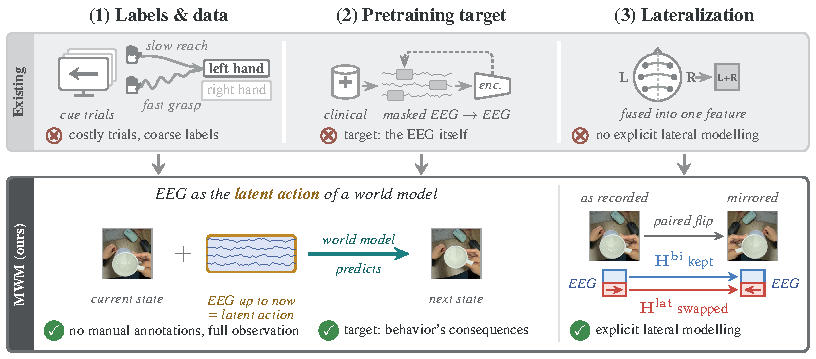
\includegraphics[width=\linewidth]{MWM/figures/mwm_teaser.pdf}
\caption{\textbf{Existing approaches (top) versus \mwm{} (bottom) on the three challenges of motor EEG representation learning.}
\textbf{(1)} Cue-based trials are costly to scale, and categorical labels give one class to movements that unfold differently~\citep{tangermann2012review,schirrmeister2017deep,lawhern2018eegnet}.
\textbf{(2)} General-purpose EEG foundation models (FMs) pretrain with EEG-only objectives~\citep{kostas2021bendr,jiang2024large,wang2025cbramod}.
\mwm{} answers both with one mechanism: it treats the EEG recorded up to the current frame as the latent action of a world model that predicts the next visual state. It therefore learns from naturalistic EEG and egocentric video without action annotations, and its target is the visual consequence of behavior rather than the EEG itself.
\textbf{(3)} Existing methods do not explicitly separate bilateral from lateral activity~\citep{schirrmeister2017deep,lawhern2018eegnet,wang2025cbramod}; \mwm{} does, and pairs each horizontal video mirror with an exchange of only the lateral component $\mathbf{H}^{\mathrm{lat}}$.}
\label{fig:mwm-teaser}
\end{figure}

Motor decoding from electroencephalography (EEG) aims to infer intended or executed movements from non-invasive recordings of brain activity. It encompasses both recognizing movement categories and estimating continuous quantities such as movement trajectories and force. This capability underpins brain--computer interfaces for assistive control and neurorehabilitation, allowing movement-related neural activity to guide external devices or rehabilitation feedback~\citep{tangermann2012review,ramos2013brain}. For these applications, useful EEG representations must capture both which movement is intended and how it unfolds, and transfer across motor tasks with limited labeled data. Learning such representations presents three challenges (Figure~\ref{fig:mwm-teaser}, top).

First, task-specific motor decoding faces limitations in both data scalability and the information conveyed by supervision. Supervised motor-decoding research is largely organized around labeled examples of predefined tasks, commonly collected through repeated, cue-based laboratory trials~\citep{tangermann2012review,schirrmeister2017deep,lawhern2018eegnet}. Such protocols make it costly to expand the volume and diversity of training data. Moreover, categorical annotations such as ``left hand'' and ``right hand'' compress motor behavior into a small vocabulary. Movements with different trajectories, speeds, or forces can share the same label, leaving their within-class variation unspecified by the training target. Direct measurements of continuous kinematics or force retain such within-class variation, but collecting them at scale typically requires task-specific instrumentation and careful synchronization with EEG. Thus, scaling motor representation learning requires both more accessible collection paradigm and supervision that retains information beyond discrete action categories.

Second, general-purpose EEG foundation models address label scarcity through self-supervised objectives such as contrastive learning, masked signal reconstruction, and neural token prediction~\citep{kostas2021bendr,chien2022maeeg,jiang2024large,wang2024eegpt,wang2025cbramod}. Although these objectives learn useful signal structure, they do not directly supervise the relationship between neural activity and movement. Their pretraining corpora are also assembled primarily for broad or clinical EEG analysis rather than for capturing continuous, naturalistic motor behavior and its consequences~\citep{jiang2024large,wang2025cbramod,obeid2016tuh,ouahidi2025reve}. These differences motivate pretraining that aligns both the learning signal and the recording context with motor decoding.

Third, motor EEG exhibits \emph{lateralization}: similar movement-related patterns can indicate different acting sides depending on which hemisphere they occur in. For example, sensorimotor rhythm suppression is often stronger over the left hemisphere for right-hand movements and vice versa~\citep{pfurtscheller1997motor,nam2011lateralization}. Without this structural prior, existing encoders~\citep{schirrmeister2017deep,lawhern2018eegnet,wang2025cbramod} must learn the relationship between patterns and hemispheric location from data, potentially requiring larger training datasets and yielding suboptimal decoding performance when data are limited.

World-model training faces a similar bottleneck in scaling data collection. Instrumented interfaces can constrain natural behavior and capture only selected aspects of action. For example, handheld grippers and motion-capture gloves primarily record hand kinematics, without directly measuring head and leg movements, interaction forces, or hand stiffness~\citep{chi2024umi,wang2024dexcap}. Video-based approaches instead infer pseudo-actions from current and future frames~\citep{bruce2024genie,gao2025adaworld}. However, access to future frames introduces a risk of target-information leakage: pseudo-actions may encode future visual content, allowing the world model to exploit prediction shortcuts rather than learn transferable action-conditioned dynamics~\citep{garrido2026lawm}.

To address these challenges, we propose the Mind World Model (\mwm{}), which jointly learns a mind model and a world model from synchronized EEG and egocentric video in EgoBrain~\citep{lin2026egobrain}. The mind model maps EEG observed up to the current frame to a latent action, and the world model uses it to predict a future visual representation. Using egocentric recordings of natural motor behavior, rather than general-purpose EEG corpora, aligns the training data with motor decoding. Visual prediction supplies supervision beyond categorical labels without task-specific annotation, enabling scalable pretraining. Encoding actions from EEG avoids explicit motion measurements and future-frame leakage. Joint learning thus produces action-related EEG representations and a world-model initialization for future prediction conditioned on real actions.

To capture motor lateralization, we introduce the Lateralization-Aware Transformer (LAT), an EEG encoder that uses frame averaging~\citep{puny2022frame} over original and mirrored representations to separate shared bilateral features from side-specific lateral features. When a video is mirrored horizontally, LAT exchanges lateral EEG features across homologous electrodes while preserving the bilateral component. This prior links corresponding movement patterns across hemispheres, reducing the burden of learning their left--right relationship from limited data.

Our contributions are as follows:
\begin{itemize}
    \item We introduce \mwm{}, which learns motor EEG representations from naturalistic EEG--video by predicting the visual consequences of behavior. This objective provides supervision beyond categorical action labels and enables scalable data collection without explicit action annotations.
    \item We propose LAT to encode hemispheric correspondence by separating bilateral and lateral EEG features, reducing the burden of learning this structure from data.
    \item We show that the pretrained world model transfers from EEG-derived actions to prediction conditioned on real actions, opening a path to scalable world-model data collection without relying on manipulation interfaces that constrain natural behavior and capture only selected aspects of action.
\end{itemize}

We evaluate the mind model on \mwmClsTasks{} classification and \mwmRegTasks{} regression tasks, and the world model on future prediction conditioned on real actions. Relative to the strongest baseline in each task family, the mind model improves task-averaged balanced accuracy by \mwmClsGainPct{}\% and Pearson correlation by \mwmRegGainPct{}\%. Ablations show that alignment, prediction, and frame averaging each improve average transfer, with effects that vary by task. Relative to the latent-action baseline, the world model reduces L1 error by \mwmWMWithinGainPct{}\% within recordings and \mwmWMSubjectGainPct{}\% on held-out subjects.

\section{Related Works}

\noindent\textbf{EEG Foundation Models.}
EEG foundation models learn transferable representations through contrastive learning, masked reconstruction, and token prediction~\citep{kostas2021bendr,chien2022maeeg,jiang2024large,wang2024eegpt}. Such objectives exploit structure in unlabeled recordings, reducing dependence on task-specific annotations and enabling transfer across EEG analysis tasks. Other work improves spatiotemporal modeling and electrode-layout flexibility~\citep{wang2025cbramod,wang2025eegmamba,doner2025luna}, scales pretraining~\citep{ouahidi2025reve}, or incorporates language and complementary neural modalities~\citep{jiang2025neurolm,xiao2025brainomni}. These advances target general EEG representation learning; \mwm{} uses visual consequences of natural behavior to supervise motor representations and explicitly models hemispheric correspondence.

\noindent\textbf{World Models.}
World models support prediction and control through observation generation~\citep{ha2018recurrent,micheli2023transformers,alonso2024diffusion} or compact latent dynamics~\citep{hafner2020dream,hansen2024tdmpc2}. Recent approaches predict frozen or jointly learned visual features~\citep{zhou2025dinowm,sobal2025rewardfree,assran2025vjepa2,maes2026leworldmodel}. Predicting in feature space lets the dynamics model focus on abstract state changes without reconstructing every detail of the observation. Video-based methods infer latent actions from frame transitions~\citep{bruce2024genie,gao2025adaworld,garrido2026lawm}. However, collecting explicit action labels can be difficult to scale, while inferring actions from future frames risks leaking target information into the action representation~\citep{garrido2026lawm}. \mwm{} pretrains a world model from EEG and video, deriving actions without explicit motion measurements or future frames. The pretrained model transfers to prediction conditioned on real actions.

\section{Method}

Our central design is to use neural activity in place of an externally recorded action within a predictive world model. The mind model observes EEG only up to the current visual state and must encode the information needed to predict what happens next. We first formulate this prediction task and its two model components, then describe the Lateralization-Aware Transformer (LAT) and training objectives.

\begin{figure}[t]
\centering
\includegraphics[width=\linewidth]{figures/mwm_overview.pdf}
\caption{\textbf{The Mind World Model.} \textbf{(a)} A frozen encoder $g$ maps the current
frame to patch features that a residual predictor advances; the same frozen $g$ builds
the target from the next frame. \textbf{(b)} The mind model encodes the EEG window, which
ends on the current frame; its LAT encoder is detailed in
Figure~\ref{fig:fliparch}. The EEG reaches the predictor only as AdaLN modulation, never as an
input token: it occupies the slot a recorded action would.}
\label{fig:mwm-framework}
\end{figure}

\subsection{Overview}

We propose the Mind World Model (\mwm{}) to jointly learn motor-related EEG representations and action-conditioned visual dynamics from synchronized EEG and egocentric video without action annotations. As illustrated in Figure~\ref{fig:mwm-framework}, \mwm{} consists of a world model and a mind model. Given an EEG segment $\mathbf{X}_t$ and a current frame $\mathbf{I}_t$, the mind model encodes the EEG into a latent action $\mathbf{a}_t$. The world model then predicts the representation of a future frame:
\begin{equation}
    \hat{\mathbf{S}}_{t+1}
    =
    p_{\phi}(\mathbf{S}_t,\mathbf{a}_t),
    \qquad
    \mathbf{S}_t=g(\mathbf{I}_t),
\end{equation}
where $g$ is a frozen image encoder and $p_{\phi}$ is a frame predictor. Future prediction both encourages the mind model to capture neural activity related to upcoming visual changes and trains the world model's dynamics and action interface.

In addition, we introduce LAT, an EEG encoder that explicitly models the lateralization of motor activity. It decomposes EEG features into bilateral and lateral components, which are respectively invariant and equivariant to swaps between homologous electrodes.

\subsection{Architecture}

A frozen visual encoder maps the current and future frames to patch tokens, and the world model advances the current token grid using a latent action encoded by LAT. Both models are trained jointly and retained separately. Motor decoders use the mind model; world-model evaluation freezes the predictor and maps IMU measurements to its action interface (Section~\ref{sec:world-action-probe}).

\subsubsection{World Model}

\paragraph{Image Encoder.}

Given a current frame $\mathbf{I}_t$ and its future frame $\mathbf{I}_{t+1}$, we use a frozen DINOv2 encoder $g$ to extract their spatial patch representations:
\begin{equation}
    \mathbf{S}_t=g(\mathbf{I}_t), \qquad
    \mathbf{S}_{t+1}=g(\mathbf{I}_{t+1}),
\end{equation}
where $\mathbf{S}_t,\mathbf{S}_{t+1}\in\mathbb{R}^{P\times D_v}$ and $P$ denotes the number of visual patches. We use patch-level features instead of a global feature because visual changes caused by hand and object movements are often spatially localized. The image encoder is kept frozen during training, providing a stable prediction target and preventing representation collapse.

\paragraph{Frame Predictor.}

The frame predictor models the transition from the current visual state to the future visual state, conditioned on EEG:
\begin{equation}
    \hat{\mathbf{S}}_{t+1}
    =
    p_{\phi}(\mathbf{S}_t,\mathbf{a}_t).
\end{equation}
We first project the EEG tokens into a compact conditioning vector $\mathbf{a}_t$. The current-frame tokens are then processed by a lightweight Transformer whose layers are modulated by $\mathbf{a}_t$ through adaptive layer normalization (AdaLN)~\citep{peebles2023scalable}:
\begin{equation}
    \operatorname{AdaLN}(\mathbf{h},\mathbf{a}_t)
    =
    \gamma(\mathbf{a}_t)\odot
    \operatorname{LN}(\mathbf{h})
    +
    \beta(\mathbf{a}_t).
\end{equation}
This design treats EEG as a latent action that controls the predicted visual transition. We further adopt residual prediction,
\begin{equation}
    \hat{\mathbf{S}}_{t+1}
    =
    \mathbf{S}_t+\Delta_{\phi}(\mathbf{S}_t,\mathbf{a}_t),
\end{equation}
such that the predictor focuses on dynamic changes instead of reconstructing the static scene.

To avoid temporal leakage, the EEG window ends at the current frame, while the prediction target is sampled from the subsequent time interval. Therefore, the target visual change is not already contained in the EEG observation window.

\subsubsection{Mind Model}

\paragraph{Transformers.}

Given an EEG segment $\mathbf{X}_t\in\mathbb{R}^{C\times T}$, we divide each channel into non-overlapping temporal patches. A channel-wise CNN embeds each patch by combining its temporal waveform and spectral representation, producing
\begin{equation}
    \mathbf{Z}_t
    =
    f_{\mathrm{emb}}(\mathbf{X}_t)
    \in\mathbb{R}^{C\times N\times D_e},
\end{equation}
where $C$ and $N$ denote the numbers of channels and temporal patches, respectively.

The EEG tokens are processed by a stack of criss-cross Transformer blocks. Each block separately performs temporal attention across patches and spatial attention across EEG channels. This factorization preserves the channel--time structure of EEG while reducing the cost of full attention. The resulting patch tokens are aggregated into the latent action $\mathbf{a}_t$ used by the frame predictor.

\begin{figure}[t]
\centering
\includegraphics[width=\linewidth]{figures/mwm_flip.pdf}
\caption{\textbf{The Lateralization-Aware Transformer (LAT) for EEG encoding.} \textbf{(a)} Patch embedding, applied within each channel,
\textbf{(b)} the learned gate $\mathbf{G}$ and the electrode permutation $\Pi$, which act
on the embedded tokens before any Transformer block, \textbf{(c)} a criss-cross block,
\textbf{(d)} frame averaging into an invariant and an equivariant feature, and
\textbf{(e)} the paired EEG--video flip. Only the learned lateral component is exchanged
across hemispheres; the raw signal is never permuted.}
\label{fig:fliparch}
\end{figure}

\paragraph{Paired Flip Augmentation and LAT.}

EgoBrain contains substantially more right-hand than left-hand movements, reflecting the natural handedness distribution of its participants. Naively training on this dataset may therefore bias the learned representation toward right-hand activity. We alleviate this imbalance through paired EEG--video flip augmentation, realised by LAT in Figure~\ref{fig:fliparch}.

Let $\Pi$ denote the permutation that exchanges homologous electrodes across hemispheres, such as C3 and C4. Instead of directly swapping the raw EEG, we learn a gate $\mathbf{G}$ that decomposes each EEG token into bilateral and lateral components:
\begin{equation}
    \mathbf{Z}^{\mathrm{lat}}
    =
    \mathbf{G}\odot\mathbf{Z},
    \qquad
    \mathbf{Z}^{\mathrm{bi}}
    =
    (1-\mathbf{G})\odot\mathbf{Z}.
\end{equation}
We define the flip operation as
\begin{equation}
    \mathcal{P}(\mathbf{Z})
    =
    \mathbf{Z}^{\mathrm{bi}}
    +
    \Pi\mathbf{Z}^{\mathrm{lat}}.
\end{equation}
Thus, bilateral activity is preserved, while lateral activity is exchanged between the two hemispheres.

For a Transformer encoder $\mathcal{T}$, we apply frame averaging over the original and flipped representations:
\begin{align}
    \mathbf{H}^{\mathrm{bi}}
    &=
    \frac{1}{2}
    \left[
    \mathcal{T}(\mathbf{Z})
    +
    \mathcal{T}(\mathcal{P}(\mathbf{Z}))
    \right], \\
    \mathbf{H}^{\mathrm{lat}}
    &=
    \frac{1}{2}
    \left[
    \mathcal{T}(\mathbf{Z})
    -
    \Pi\mathcal{T}(\mathcal{P}(\mathbf{Z}))
    \right].
\end{align}
The final EEG representation concatenates the bilateral and lateral features:
\begin{equation}
    \mathbf{H}
    =
    \left[
    \mathbf{H}^{\mathrm{bi}};
    \mathbf{H}^{\mathrm{lat}}
    \right].
\end{equation}
By construction, the bilateral component is invariant to the flip, whereas the lateral component transforms equivariantly.

During training, we randomly flip each video horizontally and apply the corresponding operation $\mathcal{P}$ to its EEG representation. This augmentation balances left- and right-oriented movements while preserving their cross-modal correspondence.

\subsection{Training Objective}

\paragraph{Alignment Loss.}

We first align the global EEG representation $\mathbf{m}_i$ with the representation $\mathbf{v}_i$ of its synchronized frame. After projection and normalization, we compute their similarities as
\begin{equation}
    s_{ij}
    =
    \frac{
    \bar{\mathbf{m}}_i^\top\bar{\mathbf{v}}_j
    }{\tau},
\end{equation}
where $\tau$ is a temperature parameter. We use a symmetric InfoNCE objective:
\begin{equation}
    \mathcal{L}_{\mathrm{align}}
    =
    \frac{1}{2}
    \left[
    \operatorname{CE}(\mathbf{S},\mathbf{y})
    +
    \operatorname{CE}(\mathbf{S}^{\top},\mathbf{y})
    \right],
\end{equation}
where $\mathbf{y}_i=i$ denotes the matched EEG--frame pair.

The global image feature is nearly invariant to horizontal flipping and therefore provides limited supervision for lateralization. We additionally construct a flip-sensitive image representation by pooling the left and right spatial regions of the image-token grid. The representations of the original and mirrored frames are used as same-sample hard negatives, encouraging the lateral EEG features to distinguish the two orientations. We denote this objective as $\mathcal{L}_{\mathrm{flip}}$.

\paragraph{Prediction Loss.}

The primary world-model objective predicts the frozen representation of the future frame. We minimize the patch-level $\ell_1$ distance:
\begin{equation}
    \mathcal{L}_{\mathrm{pred}}
    =
    \frac{1}{BP}
    \sum_{i=1}^{B}
    \sum_{p=1}^{P}
    \left\|
    \hat{\mathbf{S}}_{i,t+1}^{p}
    -
    \mathbf{S}_{i,t+1}^{p}
    \right\|_1,
\end{equation}
Because the DINOv2 encoder $g$ is frozen, the visual target remains fixed throughout training. Minimizing this loss therefore requires the mind model to extract EEG information that explains the upcoming visual transition.

The overall objective is
\begin{equation}
    \mathcal{L}
    =
    \lambda_{\mathrm{align}}\mathcal{L}_{\mathrm{align}}
    +
    \lambda_{\mathrm{flip}}\mathcal{L}_{\mathrm{flip}}
    +
    \lambda_{\mathrm{pred}}\mathcal{L}_{\mathrm{pred}}.
\end{equation}
An auxiliary masked EEG reconstruction loss can be included to preserve low-level signal information, but future-state prediction remains the defining objective of \mwm{}.

\section{Experiments}

In this section, we evaluate whether the pretrained mind model transfers to motor decoding and whether the pretrained world model transfers from EEG-derived actions to real-world action signals.

\subsection{Experimental Setup}

\paragraph{Pretraining.}
We pretrain \mwm{} on EgoBrain~\citep{lin2026egobrain}, using synchronized EEG and egocentric video from all 40 participants without downstream labels. The corpus contains 56,950 non-overlapping four-second clips, totaling 63.28 hours. Each training example contains a one-second EEG window ending at an anchor frame, the anchor frame itself, and a target frame $0.2$\,s later.

We train in FP32 using AdamW with a batch size of 128, a learning rate of $5\times10^{-4}$, weight decay of 0.05, and gradient clipping at 0.8. The learning rate follows an iteration-wise cosine schedule to $10^{-5}$ without warmup. All downstream experiments use the same fixed pretrained checkpoint.

\paragraph{Linear-probe evaluation.}
We evaluate every backbone on the same one-second EEG input sampled at 200\,Hz. We freeze the backbone in evaluation mode and train only a linear prediction head. For \mwm{}, we discard the visual encoder and frame predictor, disable stochastic flips, and flatten the frozen EEG token grid before applying the head. For regression, we additionally apply a non-affine LayerNorm and standardize each target dimension using training-split statistics.

We train the \mwm{} probes with AdamW using a learning rate of $5\times10^{-5}$, weight decay of 0.01, a batch size of 64, an iteration-wise cosine schedule to $10^{-6}$, and gradient clipping at 1. Classification probes are trained for 80 epochs with cross-entropy and 0.1 label smoothing, while regression probes are trained for 10 epochs with MSE. We select checkpoints by validation balanced accuracy for classification and validation Pearson correlation for regression. We report test balanced accuracy for classification and pooled test Pearson correlation for regression, averaging correlations across output dimensions for vector targets. All downstream results are reported as the mean and sample standard deviation over three seeds.

\paragraph{Baselines.}
We compare with BIOT, LaBraM, CBraMod, CSBrain, and REVE, using each model's channel interface and linear-probe recipe. LaBraM pretraining includes PhysioNet-MI, while REVE pretraining includes Ofner2017 and Weibo2014; the remaining reported model--dataset pairs have no known pretraining overlap.

\subsection{Regression Tasks}

\paragraph{Tasks.}
We evaluate continuous motor decoding on five tasks in Table~\ref{tab:reg-pooled-lp}. ForceGameReg predicts plateau force, SrisReachME predicts future planar reaching speed, OfnerApertureME predicts future hand-aperture change, OfnerKinME predicts future three-dimensional hand speed, and BiomechMag predicts future wrist-speed magnitude. Except for ForceGameReg, each task uses one-second EEG windows with a $0.2$\,s stride and predicts movement from $0.2$ to $0.4$\,s after the window ends.

\begin{table}[t]
\centering
\small
\setlength{\tabcolsep}{4pt}
\begin{tabular}{lccccc}
\toprule
Model & ForceGameReg & SrisReachME & OfnerApertureME & OfnerKinME & BiomechMag \\
\midrule
BIOT & 0.034{\scriptsize\,$\pm$0.017} & 0.108{\scriptsize\,$\pm$0.006} & 0.036{\scriptsize\,$\pm$0.003} & -0.019{\scriptsize\,$\pm$0.002} & 0.039{\scriptsize\,$\pm$0.001}$^{\dagger}$ \\
LaBraM & 0.107{\scriptsize\,$\pm$0.003} & 0.174{\scriptsize\,$\pm$0.003} & 0.060{\scriptsize\,$\pm$0.003} & -0.003{\scriptsize\,$\pm$0.009} & 0.119{\scriptsize\,$\pm$0.001} \\
CBraMod & 0.102{\scriptsize\,$\pm$0.007} & 0.218{\scriptsize\,$\pm$0.002} & 0.080{\scriptsize\,$\pm$0.006} & 0.073{\scriptsize\,$\pm$0.010} & 0.138{\scriptsize\,$\pm$0.001} \\
CSBrain & 0.115{\scriptsize\,$\pm$0.004} & 0.185{\scriptsize\,$\pm$0.000} & 0.047{\scriptsize\,$\pm$0.001} & 0.059{\scriptsize\,$\pm$0.013} & 0.136{\scriptsize\,$\pm$0.002} \\
REVE & 0.093{\scriptsize\,$\pm$0.023} & 0.218{\scriptsize\,$\pm$0.001} & 0.161{\scriptsize\,$\pm$0.013} & 0.187{\scriptsize\,$\pm$0.020} & 0.153{\scriptsize\,$\pm$0.005} \\
\midrule
\textbf{MWM (ours)} & \textbf{0.149{\scriptsize\,$\pm$0.025}} & \textbf{0.232{\scriptsize\,$\pm$0.009}} & \textbf{0.200{\scriptsize\,$\pm$0.051}} & \textbf{0.203{\scriptsize\,$\pm$0.013}} & \textbf{0.157{\scriptsize\,$\pm$0.002}} \\
\bottomrule
\end{tabular}
\caption{Pearson correlation, linear probe. Mean $\pm$ s.d. over 3 seeds. $^{\dagger}$On BiomechMag, BIOT uses its native-montage checkpoint, because its published bipolar montage cannot be constructed from the eight available channels.}
\label{tab:reg-pooled-lp}
\end{table}

\paragraph{Results.}
As shown in Table~\ref{tab:reg-pooled-lp}, \mwm{} achieves the highest Pearson correlation on all \mwmRegWins{} tasks. Averaged across tasks, it improves Pearson correlation by \mwmRegGainPct{}\% over the strongest single baseline.

\subsection{Classification Tasks}

\paragraph{Tasks.}
We evaluate six motor-classification tasks in Table~\ref{tab:cls-lp}: PhysioNet-MI, FineMI, Ofner2017ME, Ofner2017MI, Weibo2014, and Jeong2020. These benchmarks span both motor execution and motor imagery. All models use the same task-specific one-second interval and participant-disjoint train, validation, and test splits.

\begin{table}[t]
\centering
\small
\setlength{\tabcolsep}{4pt}
\begin{tabular}{lcccccc}
\toprule
Model & PhysioNet-MI & FineMI & Ofner2017ME & Weibo2014 & Ofner2017MI & Jeong2020 \\
\midrule
BIOT & 0.266{\scriptsize\,$\pm$0.007} & 0.172{\scriptsize\,$\pm$0.009} & 0.149{\scriptsize\,$\pm$0.020} & 0.161{\scriptsize\,$\pm$0.003} & 0.147{\scriptsize\,$\pm$0.005} & 0.097{\scriptsize\,$\pm$0.003} \\
LaBraM & 0.447{\scriptsize\,$\pm$0.012} & 0.179{\scriptsize\,$\pm$0.014} & 0.160{\scriptsize\,$\pm$0.008} & 0.185{\scriptsize\,$\pm$0.020} & 0.158{\scriptsize\,$\pm$0.001} & 0.118{\scriptsize\,$\pm$0.008} \\
CBraMod & 0.587{\scriptsize\,$\pm$0.006} & 0.199{\scriptsize\,$\pm$0.002} & 0.177{\scriptsize\,$\pm$0.026} & 0.183{\scriptsize\,$\pm$0.002} & 0.147{\scriptsize\,$\pm$0.003} & 0.146{\scriptsize\,$\pm$0.000} \\
CSBrain & 0.552{\scriptsize\,$\pm$0.009} & 0.183{\scriptsize\,$\pm$0.002} & 0.174{\scriptsize\,$\pm$0.008} & 0.162{\scriptsize\,$\pm$0.001} & 0.148{\scriptsize\,$\pm$0.005} & 0.149{\scriptsize\,$\pm$0.006} \\
REVE & 0.562{\scriptsize\,$\pm$0.001} & 0.190{\scriptsize\,$\pm$0.004} & 0.187{\scriptsize\,$\pm$0.009} & 0.186{\scriptsize\,$\pm$0.008} & 0.154{\scriptsize\,$\pm$0.001} & 0.138{\scriptsize\,$\pm$0.004} \\
\midrule
\textbf{MWM (ours)} & \textbf{0.599{\scriptsize\,$\pm$0.005}} & \textbf{0.200{\scriptsize\,$\pm$0.005}} & \textbf{0.202{\scriptsize\,$\pm$0.007}} & \textbf{0.187{\scriptsize\,$\pm$0.005}} & \textbf{0.165{\scriptsize\,$\pm$0.002}} & \textbf{0.158{\scriptsize\,$\pm$0.004}} \\
\bottomrule
\end{tabular}
\caption{Classification accuracy, linear probe. Mean $\pm$ s.d. over 3 seeds.}
\label{tab:cls-lp}
\end{table}

\paragraph{Results.}
As shown in Table~\ref{tab:cls-lp}, \mwm{} achieves the highest balanced accuracy on all \mwmClsWins{} tasks. Averaged across tasks, it improves balanced accuracy by \mwmClsGainPct{}\% over the strongest single baseline.

\subsection{World Models}
\label{sec:world-action-probe}

We evaluate the pretrained world models by mapping synchronized IMU measurements to their frozen action interfaces. We train the same lightweight IMU adapter for each model and predict frozen DINOv2 features $0.2$\,s ahead under within-recording and held-out-subject splits.

\paragraph{Baselines and Evaluation.}
We compare \mwm{} with a predictor pretrained using inverse-dynamics latent actions~\citep{garrido2026lawm} and a randomly initialized predictor. All models use the same inputs, targets, predictor architecture, IMU-adapter architecture, and $128$-dimensional action interface. We report L1 error, cosine similarity, and the increase in error after shuffling the IMU actions.

\begin{table}[ht]
\small
\setlength{\tabcolsep}{4pt}
\caption{IMU action probing on held-out next-step prediction. All pretrained models use the same predictor and a $128$-dimensional action interface.}
\label{tab:wm-probe}
\begin{center}
\begin{tabular}{lcccccc}
\toprule
& \multicolumn{3}{c}{Within recording}
& \multicolumn{3}{c}{Held-out subjects} \\
\cmidrule(lr){2-4}\cmidrule(lr){5-7}
Model & L1$\downarrow$ & Cos.$\uparrow$ & $\Delta_{\mathrm{act}}\uparrow$
& L1$\downarrow$ & Cos.$\uparrow$ & $\Delta_{\mathrm{act}}\uparrow$ \\
\midrule
\textbf{\mwm{} (ours)} & 0.5009 & 0.8773 & \textbf{+0.0079} & \textbf{0.4933} & 0.8850 & \textbf{+0.0057} \\
% Hand action & \textbf{0.5004} & 0.8776 & +0.0068 & -- & -- & -- \\
Latent action & 0.6520 & 0.8463 & +0.0020 & 0.5543 & 0.8737 & +0.0029 \\
Random init. & 0.7334 & 0.8334 & +0.0000 & 0.7224 & 0.8407 & +0.0000 \\
% Copy frame & 0.5036 & \textbf{0.8783} & -- & 0.4961 & \textbf{0.8859} & -- \\
\bottomrule
\end{tabular}
\end{center}

\end{table}

\paragraph{Results.}
Table~\ref{tab:wm-probe} shows that \mwm{} achieves lower L1 error and a larger action gap than the latent-action model on both splits. Relative to the latent-action model, these L1 errors represent reductions of \mwmWMWithinGainPct{}\% within recordings and \mwmWMSubjectGainPct{}\% on held-out subjects. The randomly initialized predictor has a zero action gap, whereas \mwm{} remains sensitive to matched IMU actions on both splits.

\section{Conclusion}

We introduced \mwm{}, which uses EEG as the latent action of a world model to learn motor representations without explicit action annotations. The Lateralization-Aware Transformer incorporates hemispheric correspondence through frame averaging. Relative to the strongest baseline in each task family, the mind model improves task-averaged balanced accuracy by \mwmClsGainPct{}\% and Pearson correlation by \mwmRegGainPct{}\%, while the world model supports future prediction conditioned on real actions. These results support synchronized neural and visual experience as supervision for motor decoding and world modeling.

\noindent\textbf{Limitations.} Our world-model evaluation tests action-conditioned prediction error; establishing end-to-end evaluation, such as robotic planning, remains future work.


\chapter{Learning Graph Search Heuristics}
\label{chapter:phil}

Chapter~\ref{chapter:mwm} grounds action meaning by jointly learning how EEG-derived latent actions predict visual consequences. To complete a task, however, a person may wish to specify the desired result rather than each action. This chapter and Chapter~\ref{chapter:dysta} therefore move from the action level to the goal level, studying complementary planning and policy approaches. In the dissertation's embodiment framing, the goal input for \phil{} is an image depicting a desired outcome, corresponding to the visual output studied in Part~\ref{part:bridge}. To use that goal in graph search, the depicted outcome must be represented by a goal node and its features in a state graph. \phil{} then guides the search from a start node toward that goal. The evaluations in this chapter study supplied graph-and-goal problems; grounding decoded goal images in planner states remains a future integration step.

\phil{} (Path Heuristic with Imitation Learning) learns a graph neural network heuristic that predicts node-to-goal distances using both local structure and a memory of the graph explored so far. This heuristic guides search toward promising states and reduces the number of expansions required to find a path. The chapter evaluates this approach on grid environments, graphs from several domains, and simulated indoor UAV path planning. Chapter~\ref{chapter:dysta} studies the complementary language-instruction interface, corresponding to the text output of Part~\ref{part:bridge}: a visual policy generates actions directly from that instruction and observation history. Together, the two chapters link image-specified and language-specified goals to complementary search-based and policy-based approaches.

\section{Introduction}
\label{sec:intro}

%\jure{The paper is great! It reads very nicely and is very thoroughly and accurately written. Great job!! I left quite some comments but don't worry about them. They are all optional. :) }

%\jure{ Here are a few high-level comments and observations:\\
%1) Method is described very densely and it takes quite a bit of staring at the paper and connecting different parts to get what is going on. I would suggest taking a bit more space and being a bit more verbose in the method description.\\
%2) Experiments are extensive but some parts feel like a bit too much detail (hyperparameters, baseline settings, etc.). I think we can move those details to the supp materials and then use this space to expand on the method.\\
%3) When we describe experimental results, let's say "PHIL outperfosm method X by 40\% on average". Let's quantify and summarize the performance improvement. Saying "PHIL wins everywhere except in this one case" is actually putting emphasis on the one case rather than to put emphasis on how great our method is.\\}

Search heuristics are essential in several domains, including robotics, AI, biology, and chemistry \cite{bhardwaj2017learning, chen2020retro, gebser2013domain, mac2016heuristic, sharma2017identifying, yeh2012pathway}. For example, in robotics, complex robot geometries often yield slow collision checks, and search algorithms are constrained by the robot's onboard computation resources, requiring well-performing search heuristics that visit as few nodes as possible~\cite{bhardwaj2017learning, mac2016heuristic}. In AI, domain-specific search heuristics are useful for improving the performance of inference engines operating on knowledge bases \cite{gebser2013domain, sharma2017identifying}. Search heuristics have been previously also developed to reduce search efforts in protein-protein interaction networks \cite{yeh2012pathway} and in planning chemical reactions that can synthesize target chemical products \cite{chen2020retro}. This broad set of applications underlines the importance of good search heuristics that are applicable to a wide range of problems. 


%\jure{Number of examples here is long, perhaps we can cut one or two to save space.} \update{Removed game dev and b\&b}


%We formulate finding search heuristics as an optimization process, allowing practitioners to quickly find useful search heuristics. We illustrate this concept in Figure \ref{fig:money-fig}.

\begin{figure}[!htpb]
\centering
\includegraphics[width=0.9\textwidth]{figures/money_fig.png}
\caption{The goal is to navigate (find a path) from the start to the goal node. While BFS visits many nodes to find a start-to-goal path (left), one can use a heuristic based on the features of the nodes (e.g., Euclidean distance) on the graph to reduce the search effort (middle). We propose \alg to learn a tailored search heuristic for a given graph, capable of reducing the number of visited nodes even further by exploiting the inductive biases of the graph (right). }
\label{fig:money-fig}
\end{figure}

The search task can be formulated as a pathfinding problem on a graph, where given a graph, the task is to navigate and find a short feasible path from a start node to a goal node, while in the process visiting as few nodes as possible (Figure~\ref{fig:money-fig}). The most straightforward approach would be to launch a search algorithm such as breadth-first search (BFS) and iteratively expand the graph from the start node until it reaches the goal node. Since BFS does not harness any prior knowledge about the graph, it usually visits many nodes before reaching the goal, which is expensive in cases such as robotics where visiting nodes is costly. To visit fewer nodes during the search, one may use domain-specific information about the graph via a \textit{heuristic} function \cite{pearl1984heuristics}, which allows one to define a distance metric on graph nodes to prune directions that seem less promising to explore. Unfortunately, coming up with good search heuristics requires significant domain expertise and manual effort.
%, without straightforward ways to further refine proposed heuristics. 

While there has been significant progress in designing search heuristics, it remains a challenging problem. Classical approaches \cite{khalidi2020t, adabala2020multi} tend to hand-design search heuristics, which requires domain knowledge and a lot of trial and error. To alleviate this problem, there has been significant development in general-purpose search heuristics based on trading-off greedy expansions and novelty-based exploration \cite{xie2012planning, xie2014adding, lipovetzky2017best, teichteil2021boundary} or search problem simplifications \cite{bonet2001planning, zhu2003landmark, richter2010lama}. These approaches alleviate some of the common pitfalls of goal-directed heuristics, but we demonstrate that if possible, it is useful to learn domain-specific heuristics that can better exploit problem structure.

On the other hand, learning-based methods face a set of different challenges. Firstly, the data distribution is not i.i.d., as newly encountered graph nodes depend on past heuristic values, which means that supervised learning-based methods are not directly applicable. Secondly, heuristics should run fast, with ideally constant time complexity. Otherwise, the overall asymptotic time complexity of the search procedure could be increased. Finally, as the environment (search graph) sizes increase, reinforcement learning-based heuristic learning approaches tend to perform poorly \cite{bhardwaj2017learning}. State-of-the-art imitation learning-based methods can learn useful search heuristics \cite{bhardwaj2017learning}; however, these methods still rely on feature-engineering for a specific domain and do not generally guarantee a constant time complexity with respect to graph sizes.


\begin{figure}[h]
\centering
\includegraphics[width=0.9\textwidth]{figures/method_figure2.pdf}
\caption{Main components of \alg: On the left, using a greedy mixture policy induced by the current version of our parameterized heuristic $h_\theta$ and an oracle heuristic $h^*$ (i.e., a heuristic that correctly determines distances between nodes), we roll-out a search trajectory from the start node to the goal node. Each trajectory step contains a set of newly added fringe nodes with bounded random subsets of their 1-hop neighborhoods and their oracle ($h^*$) distances to the goal node. Trajectories are aggregated throughout the training procedure. On the right, we use truncated backpropagation through time on each collected trajectory to train $h_\theta$, where $\hat{h}$ is the predicted distance between $x_2$ and $x_g$, and $z_2$ is the updated state of the memory. Here, the memory captures the embedding of the graph visited so far.}
\label{fig:approach-high-level}
\end{figure}

%\jure{Here we say ``memory'', can we continue the sentence to explain what memory is. Something like: , which captures the graph visited so far.} \update{Added a short sentence at the end}
%\jure{Questions:\\
%-- what is "aggregate dataset"? So far we just explained that there is a graph, a start and a goal node. We need to explain what "aggregate dataset" is or change the label.\\
%-- can we use the concepts introduce in the main text in this figure as well.\\
%-- why do we label $x_{end}$? shouldn't we call it $x_{g}$. Let's use consistent terminology. Also $d_gt$ can we define it.\\
%-- Basically, if we use symbols in the figure, let's define them in the caption.}

%We formulate finding search heuristics as an optimization process, allowing practitioners to quickly find useful search heuristics. We illustrate this concept in Figure \ref{fig:money-fig}.


In this paper, we propose \textit{Path Heuristic with Imitation Learning} (\alg), a framework that extends the recent imitation learning-based heuristic search paradigm with a learnable \textit{explored graph memory}. This means that \alg learns a representation that allows it to capture the structure of the so far explored graph, so that it can then better select what node to explore next (Figure \ref{fig:approach-high-level}).  We train our approach to predict the node-to-goal distances ($h^{*}$ in Figure \ref{fig:approach-high-level}) of graph nodes during search. To train our memory module, which captures the explored graph, we use truncated backpropagation through time (TBTT) \cite{sutskever2013training}, where we utilize ground-truth node-to-goal distances as a supervision signal at each search step. Our TBTT procedure is embedded within an adaptation of the AggreVaTe imitation learning algorithm \cite{ross2014reinforcement}. \alg also includes a \textit{specialized graph neural network architecture}, which allows us to apply \alg to diverse graphs from different domains.

%\jure{Here we introduce many concepts: like ``explored graph'', ``memory module'', ``TBTT'', ``cost-to-go'', ... Can we please make sure to use these concepts in Fig 2 (have some part of the figure labeled using these labels.}

%Figure \ref{fig:approach-high-level} presents the high-level idea of our approach. 

We evaluate \alg on standard benchmark heuristic learning datasets (Section \ref{sec:experiments-grids}), diverse graph-based datasets from different domains (Section \ref{sec:experiments-diversity}), and practical UAV flight use cases (Section \ref{sec:experiments-drone}). Experiments demonstrate that \alg outperforms state-of-the-art heuristic learning methods up to $4 \times$. Further, \alg performs within $4.9 \%$ of an oracle in indoor drone planning scenarios, which is up to a $21.5 \%$ reduction compared with commonly used approaches. In practice, our contributions enable practitioners to quickly extract useful search heuristics from their graph datasets without any hand-engineering.
\section{Preliminaries}
\label{sec:prelims}
\xhdr{Graph search} Suppose that we are given an unweighted connected graph $\mathcal{G} = (\VS, \mathcal{E})$, where $\VS$ is a set of nodes, and $\mathcal{E}$ a corresponding set of edges. Further suppose that each node $i \in \VS$ has corresponding features $x_i \in \mathbb{R}^{D_v}$, and each edge $(i, j) \in \mathcal{E}$ has features $e_{ij} \in \mathbb{R}^{D_e}$. Assume that we are also given a start node $v_s \in \VS$ and a goal node $v_g \in \VS$. At any stage of our search algorithm, we can partition the nodes of our graph into three sets as $\VS = \text{CLOSE} \cup \text{OPEN} \cup \text{REST}$, where CLOSE are the nodes already explored,  $\text{OPEN}$ are candidate nodes for exploration (i.e., all nodes connected to any node in CLOSE, but not yet in CLOSE), and $\text{REST}$ is the rest of the graph. Each \textit{expansion} moves a node from $\text{OPEN}$ to CLOSE, and adds the neighbors of the given node from $\text{REST}$ to $\text{OPEN}$. We call the set of newly added fringe nodes $\VS_{new}$ at each search step.  At the start of the search procedure, $\text{CLOSE} = \{v_s\}$ and we expand the nodes until $v_g$ is encountered (i.e., until $v_g \in \text{CLOSE}$).

\xhdr{Greedy best-first search} We can perform \textit{greedy best-first search} using a greedy fringe expansion policy, such that we always expand the node $v \in \text{OPEN}$ that minimizes $h(v, v_g)$. Here, $h : \VS \times \VS \longrightarrow \mathbb{R}$ is a tailored heuristic function for a given use case. In our work, we are interested in learning a function $h$ that predicts shortest path lengths, this way minimizing $|\text{CLOSE}|$ in a \textit{greedy best-first search} regime.

%\update{Best-first should be clearer now - also organized this section a bit more}


%jure{We never define what a clairvoyant oracle is. Isn't oracle already optimal/supernatural/} \update{We decide to just use oracle for symbol brevity and it's easier to understand.}
\xhdr{Imitation of perfect heuristics} Partially observable Markov decision processes (POMDPs) are a suitable framework to describe the problem of learning search heuristics~\cite{bhardwaj2017learning}. We can have $s = (\text{CLOSE}, \text{OPEN}, \text{REST})$ as our state, an action $a \in \mathcal{A}$ corresponds to moving a node from $\text{OPEN}$ to CLOSE, and the observations $o \in \mathcal{O}$ are the features of newly included nodes in $\text{OPEN}$. Note that one could consider an MDP framework to learn heuristics, but the time complexity of operating on the whole state is in most cases prohibitive. We also define a history $\psi \in \Psi$ as a sequence of observations $\psi = o_1, o_2, o_3, ...$. Our work leverages the observation that using a heuristic function during greedy best-first search that correctly determines the length of the shortest path between fringe nodes and the goal node will also yield minimal $|\text{CLOSE}|$. For training, we adopt a perfect heuristic $h^{*}$, similar to \cite{bhardwaj2017learning}, which has full information about $s$ during search. Such oracle can provide ground-truth distances $h^{*}(s, v, v_g)$, where $v \in \text{OPEN}$. To conclude, we define a \textit{greedy best-first search policy} $\pi_{\theta}$ that uses a parameterized heuristic $h_{\theta}$ to expand nodes from $\text{OPEN}$ with minimal heuristic values. One could also directly use a POMDP solver for the above-described problem, but this approach is usually infeasible due to the dimensionality of the search state \cite{choudhury2017adaptive}.

%\update{Policy defined}

%Consider a partially observable Markov decision process (POMDP) defined by an 8-tuple $(S, A, R, P, \Omega, O, \gamma, \rho_0)$. In this POMDP definition, we have $S$ being a set of valid states, $A$ set of valid actions, $R : S \times A \longrightarrow \mathbb{R}$ the reward function, $P : S \times A \longrightarrow \mathcal{P}(S)$ the transition probability function, $\rho_0$ the initial state distribution, $\gamma \in [0, 1]$ the discount factor, $\Omega$ the set of observations, and $O : S \times A \longrightarrow \mathcal{P}(\Omega)$ a conditional observation probability function. We can also define a history $\psi \in \Psi$ as a sequence of observations $\psi = o_1, o_2, o_3, ...$. In general, our goal is to find an action policy $\pi(\cdot | \psi)$ that maximizes expected discounted rewards under the induced trajectory distribution. 

\section{Related Work}

\xhdr{General purpose heuristic design} There has been significant research in designing general-purpose heuristics for speeding up satisficing planning. The first set of approaches are based on simplifying the search problem for example using landmark heuristics \cite{bonet2001planning, richter2010lama}. The next set of approaches aim to include novelty-based exploration in greedy best-first search \cite{xie2012planning, xie2014adding, lipovetzky2017best, teichteil2021boundary}. The latter set of approaches showed state-of-the-art performance (best-first width search \cite{lipovetzky2017best, teichteil2021boundary}, BFWS) in numerous settings. We show that in domains where data is available, it can be more effective to incorporate a learned heuristic into a greedy best-first search procedure.


\xhdr{Learning heuristic search} There have been numerous previous works that attempt to learn search heuristics: Arfaee \etal \cite{arfaee2011learning} propose to improve heuristics iteratively, Virseda \etal  \cite{us2013learning} learn to combine heuristics to estimate graph node distances, Wilt \etal \cite{wilt2015building} and Garrett \etal \cite{garrett2016learning} propose to learn node rankings, Thayer \etal \cite{thayer2011learning} suggest to infer heuristics during a search, and Kim \etal \cite{KimA20} train a neural network to predict graph node distances. These methods generally do not consider the non-i.i.d. nature of heuristic search. Further, Bhardwaj \etal \cite{bhardwaj2017learning} propose \sail, where heuristic learning is framed as an imitation learning problem with cost-to-go oracles. The \sail heuristic uses hand-designed features tailored for obstacle avoidance, with a linear time-complexity in the number of explored grid nodes found to be colliding with an obstacle. Feature-engineering becomes more difficult as we attempt to learn heuristics on diverse graphs such as ones seen in Section \ref{sec:experiments-diversity}, where we may need expert knowledge. Further, heuristics that do not have a constant time complexity in the size of the graph \cite{bhardwaj2017learning, ariki2019fully, terasawa20203d, yonetani2020path, archetti2021neural} generally scale poorly with graph size and hence have constrained use cases. Recent approaches to learning heuristics include Retro* \cite{chen2020retro} by Chen \etal, where a heuristic is learned in the context of AND-OR search trees for chemical retrosynthetic planning. Our work focuses on a more general graph setting.

There has been significant progress on learning heuristics for NP-hard combinatorial optimization problems \cite{NIPS2017_d9896106, NEURIPS2018_8d3bba74, NEURIPS2020_49f85a9e}. Focusing on solving NP-hard problems allows these approaches to design algorithms that are often non-exact and have a relatively large computational budget. This is not the case for methods that focus on polynomial time search, where learning-based methods are bounded by the determinism and time complexity of classical algorithms such as greedy best-first search.



%Still, these heuristic learning methods, due to their time complexities, are impractical for the application in polynomial-time search problems, on which this work focuses.

%\textbf{\phil generally runs in $\mathcal{O}(1)$ per prediction without requiring any hand-engineering. We provide a comprehensive comparison with \sail in Section \ref{sec:experiments-grids}.}

%recent works by Ariki \etal \cite{ariki2019fully} and Teresawa \etal \cite{terasawa20203d} perform convolutions over full-graphs to infer their heuristic values, which  


\xhdr{Learning general purpose search} 
Learning general search policies is a very well-studied research area with a rich set of developments and applications. These include Monte Carlo Tree Search methods \cite{silver2010monte, guez2018learning}, implicit planning methods \cite{deac2020xlvin, karkus2017qmdp, tamar2016value}, and imagination-based planning approaches \cite{pascanu2017learning, weber2017imagination}. Learning search heuristics can be seen as a special case of \textit{general purpose search}, where the search problem is treated as a partially observable Markov decision process with restricted action evaluation (see Section \ref{sec:approach}), and with models running in $\mathcal{O}(1)$ to remain competitive time-complexity-wise on problems where best-first search performs well. \textit{General purpose search} methods do not take into account the above-mentioned constraints, which motivates the development of tailored approaches for learning heuristics \cite{ bhardwaj2017learning, chen2020retro}.

%\jure{I am not sure what precisely are we trying to say here and how does our method relate/differ from this} \update{The goal here was to answer the question of 'why not just use MCTS or something implicit like VIN'. I tried to rephrase the paragraph so that it is clear. I am also happy to drop this in case you think it is not necessary.}

\xhdr{Imitation learning} Our approach builds on prior work in imitation learning (IL) with cost-to-go oracles. Cost-to-go oracles have been incorporated in the context of IL in methods such as SEARN \cite{daume2009search}, AggreVaTe \cite{ross2014reinforcement}, LOLS \cite{chang2015learning}, AggrevaTeD \cite{sun2017deeply}, DART \cite{laskey2017dart}, and THOR \cite{sun2018truncated}. \sail \cite{bhardwaj2017learning} presents an AggreVaTe-based algorithm for learning heuristic search. We extend \sail by incorporating a recurrent $Q$-like function, in which sense our algorithm more closely resembles AggreVaTeD by Sun \etal \cite{sun2017deeply}. While a recurrent policy can be easily incorporated in AggreVaTeD, we cannot use a policy to evaluate actions. This is due to the fact that we would either have to evaluate all actions in a state, which is computationally infeasible, or we would have to give up on taking actions that are not in the most recent version of the search fringe, which would degrade the performance (see Section \ref{sec:approach}). %RNNs have been previously incorporated in SEARNN by Leblond \etal \cite{searnn} in the context of structured prediction, however we focus on imitation of cost-to-goal oracles. 

%nstead, we propose to use backpropagation through time on the roll-out phase of our algorithm, with cost-to-go supervision on each time step.
\section{Path Heuristic with Imitation Learning}
\label{sec:approach}

%\jure{Notice notation here is using $v_s$, $v_g$, where s is start and t is target. This is not consistent with introduction. Let's fix intro to use the same terminology.}

\xhdr{Training objective} With the aim of minimizing $|\text{CLOSE}|$ after search, our goal is to train a parameterized heuristic function $h_{\theta} : \Psi \times \VS \times \VS \longrightarrow \mathbb{R}$ to predict ground-truth node distances $h^{*}$ and use $h_\theta$ within a greedy best-first policy $\pi_\theta$ at test time.  More specifically, we assume access to a distribution over graphs $P_{\mathcal{G}}$, a start-goal node distribution $P_{v_{sg}}(\cdot \: | \: \mathcal{G})$, and a time horizon $T$. Moreover, we assume a joint state-history distribution $s, \psi \sim P_s(\cdot \: | \: \mathcal{G}, t, \pi_{\theta}, v_s, v_g)$, where $P_s$ represents the probability our search being in state $s$, at time $0 \leq t \leq T$ on graph $\mathcal{G}$ with pathfinding problem $(v_s, v_g)$, with a greedy best-first search policy $\pi_{\theta}$ using heuristic $h_{\theta}$. Hence, our goal can be summarized as minimizing the following objective:

\begin{equation}
    \label{eq:obj}
    \mathcal{L}(\theta) = \mathop{\EX}_{\substack{\mathcal{G} \sim P_{\mathcal{G}}, \\ (v_s, v_g) \sim P_{v_{sg}} \\ t \sim \mathcal{U}(0, ..., T), \\ s, \psi \sim P_s}}\big[\frac{1}{|\text{OPEN}|}\sum_{v \in \text{OPEN}} (h^{*}(s, v, v_g) - h_{\theta}(\psi, v, v_g))^{2} \big]
\end{equation}

Before we describe the algorithm that can be used to minimize $\mathcal{L}$, we rewrite $h_{\theta}$ to include a memory digest component ($z_t$), which represents an embedding of $\psi$ at time step $t$. Hence, $h_\theta$ becomes $h_{\theta} : \mathbb{R}^{d} \times \mathcal{O} \times \VS \times \VS \longrightarrow \mathbb{R}$, where $d$ is the dimensionality of our memory's embedding space. As opposed to previous methods \cite{bhardwaj2017learning}, $z_{t}$ allows us to \textit{automatically extract} relevant features for heuristic computations and concurrently \textit{reduce the computational complexity} of the heuristic function. Further, as shown in \cite{bhardwaj2017learning}, if we would use $h_{\theta}$ to evaluate all actions in a state (i.e., recalculate the heuristic values of all nodes in $\text{OPEN}$), we would need a squared reduction in the number of expanded nodes compared with BFS for \phil to bring performance benefits over BFS, which however may not be possible on all datasets. Hence, we constrain the heuristic only to evaluate new $\text{OPEN}$ nodes which we obtain after moving a node to $\text{CLOSE}$, calling the set of new fringe nodes $\VS_{new}$ after each expansion. In practice, the policy $\pi_{\theta}$  yields an algorithm equivalent to greedy best-first search, with the heuristic function replaced by $h_{\theta}$.

%\jure{This is the first time we define policy $\pi$ and it is unclear that it actually refers to our work PHIL}  \update{Should be clearer now: $\pi_{\theta}$ mentioned at the beginning of approach and in background}

\subsection{Learning algorithm \& architecture}
\label{sec:ila}

\begin{algorithm}[t]
	\caption{\phil --- Sequential Heuristic Training}\label{alg:il_alg}
	Obtain hyperparameters $T$, $\beta_{0}$, $N$, $m$, $t_\tau$;\\
	Initialize $\mathcal{D} \leftarrow \emptyset$, $h_{\theta_{1}}$; \\ \label{lst:line:}
	\For{$i = 1, \ldots, N$}
	{   Sample $\mathcal{G} \sim P_{\mathcal{G}}$; \\
	    Sample $v_s, v_g \sim P_{v_{sg}}$; \\
	    Set $\beta \leftarrow \beta_0^{i}$; \\
        Set mixture policy $\pi_{mix} \leftarrow (1 - \beta) * \pi_{\theta_{i}} + \beta  * \pi^{*}$; \\
	    Collect $m$ trajectories $\tau_{ij}$ as follows; \\
		\For{$j = 1,\ldots,m$}
		{   
			Sample $t \sim \mathcal{U}(0, ..., T - t_{\tau})$;\\
			Roll-in $t$ time steps of $\pi_{\theta_{i}}$ to obtain $z_t$ and new state $s_t = (\text{CLOSE}^{0}, \text{OPEN}^{0}, \text{REST}^{0})$; \\
			Roll-out trajectory $\tau_{ij}$ as follows;\\
			\For{$k = 1,\ldots, t_{\tau}$}
		    {   
    			Update $s_{t + k - 1}$ using $\pi_{mix}$ to get new state $s_{t+k}$ and new fringe state $\text{OPEN}^{k}$; \\
    			Obtain new fringe nodes $\VS_{new} = \text{OPEN}^{k} \setminus \text{OPEN}^{k-1}$; \\
    			Update trajectory $\tau_{ij} \leftarrow \tau_{ij} \cup \{(\VS_{new}, h^{*}(s_{t+k}, \VS_{new}, v_g))\}$; \\
	        }
		    Update dataset $\mathcal{D} \leftarrow \mathcal{D} \cup \{(\tau_{ij}, z_t)\}$ or $\mathcal{D} \cup \{(\tau_{ij}, 0)\}$; \\	
	    }
	    Train $h_{\theta_{i}}$ using TBTT on each $\tau \in \mathcal{D}$ to get $h_{\theta_{i+1}}$;\\  
	}
	\Return{best performing $h_{\theta_{i}}$ on validation};
\end{algorithm}


% Describe algo
\xhdr{Imitation learning algorithm} In Algorithm \ref{alg:il_alg}, we present the pseudo-code of the IL algorithm used to train our heuristic models (Figure \ref{fig:il-proc}). The high-level idea of our algorithm is that we aggregate trajectories of search traces (i.e., sequences of new fringe nodes) and use truncated backpropagation through time to optimize $h_{\theta}$ after each data-collection step. In particular, after sampling a graph $\mathcal{G}$ and a search problem  $v_s, v_g$, we use our greedy learned policy $\pi_\theta$ induced by $h_\theta$ to roll-in for $t \sim \mathcal{U}(0, \dots, T - t_{\tau})$ expansions, where $T$ is the episode time horizon, and $t_\tau$ is the roll-out length. From our roll-in, we obtain a new state $s = (\text{CLOSE}^{0}, \text{OPEN}^{0}, \text{REST}^{0})$, and an initial memory state $z_t$. After our roll-in, we roll-out for $t_{\tau}$ steps using our mixture policy $\pi_{mix}$, which is obtained by probabilistically blending $\pi_\theta$ and the greedy best-first policy induced by the oracle heuristic $\pi^{*}$. In a roll-out, we collect sequences of new fringe nodes, together with their ground-truth distances to the goal $v_g$, given by $h^{*}$.  Once the roll-out is complete, we append the obtained trajectory and the initial state for the following optimization using backpropagation through time. Further analysis on the trade-offs between using rolled-in states $z_t$ or zeroed-out states for training can be found in the supplementary material.

Note that we could also use supervised learning-based approaches to sample a fixed dataset of ($v_s$, $v_g$, $h^{*}(s, v_s, v_g)$) 3-tuples and train a model to predict node distances conditioned on their features. However, our experiments in Section \ref{sec:experiments} demonstrate that ignoring the non-i.i.d. nature of heuristic search negatively impacts model performance, with supervised learning-based methods performing up to $40 \times$ worse.


%\jure{As one is reading this, the question besomese, why not just sample some paths, and learn a MLP or GNN in the IID setting to predict the shortest path distance from current node to goal. It would be good to have a quick paragraph here discussing why this is not a good idea and a forward pointer to experiments/ablations which show that imitation learning gives x\% improvement over IID learning.} \update{Wrote a short paragraph about this.}

\begin{figure}[!htpb]
    \centering
    \includegraphics[width=0.9\textwidth]{figures/method_fig.png}
    \caption{This figure demonstrates the core idea behind our IL algorithm. We present the roll-in phase on the left-hand side, where our policy is rolled in for $t$ steps to obtain state $s_t$ and embedding $z_t$. On the right-hand side, we show the trajectory collection and training steps, where we aggregate the trajectory for downstream training (green) and use truncated backpropagation through time on the collected dataset (red).
    }
    \label{fig:il-proc}
    
\end{figure}

\begin{wrapfigure}[12]{R}{0.55\textwidth}
    \begin{algorithm}[H]
    	\caption{Heuristic func. ($h_\theta$) forward pass}\label{alg:htheta_alg}
    	 Obtain $x_i, x_j (j \in \mathcal{N}_i), e_{ij}, x_g$ $z_t$;\\
    	 $x_i \leftarrow f(x_i, x_g, D_{EUC}(x_i, x_g), D_{COS}(x_i, x_g)$);\\
     	 $x_j \leftarrow f(x_j, x_g, D_{EUC}(x_j, x_g), D_{COS}(x_j, x_g)$); \\
    
    	 $g_i \leftarrow \phi(x_i, \mathop{\oplus_{j \in \mathcal{N}_i}} \gamma(x_i, x_j, e_{ij}))$;\\
         $g^{\prime}_i, z_{i, t+1} \leftarrow \textsc{GRU}(g_i, z_t)$;\\
    	 $z_{t+1} \leftarrow \overline{z_{i, t+1}}$;\\ 
    	 $\hat{h}_i \leftarrow \textsc{MLP}(g^{\prime}_i, x_g);$\\
    	\Return{$\hat{h}_i ,z_{t+1}$};\\
    \end{algorithm}
\end{wrapfigure}


\textbf{Recurrent GNN architecture.} In each forward pass, $h_{\theta}$ obtains a set of new fringe nodes $\VS_{new}$, the goal node $v_g$, and the memory $z_t$ at time step $t$. We represent each node in $\VS_{new}$ using its features $x_{i} \in \mathbb{R}^{D_v}$, and likewise the goal node $v_g$ using its features $x_{g} \in \mathbb{R}^{D_v}$. Further, for each $i \in \VS_{new}$, we uniformly sample an $n \in \mathbb{N}_{\geq 0}$ bounded set of nodes present in the 1-hop neighborhood of $i$, calling this set $\mathcal{N}_i$, with $|\mathcal{N}_i| \leq n$. This sampling step produces a set of neighboring node features, where each $j \in \mathcal{N}_i$ has features $x_{j} \in \mathbb{R}^{D_v}$, and corresponding edge features $e_{ij} \in \mathbb{R}^{D_e}$.

%Further, for each $i \in \VS_{new}$, we uniformly sample up to $n \in \mathbb{N}_{\geq 0}$ nodes from the 1-hop neighborhood of $i$. This produces a bounded set of nodes $\mathcal{N}_i$, where $|\mathcal{N}_i| \leq n$, each $j \in \mathcal{N}_i$ has features $x_{j} \in \mathbb{R}^{D_v}$, and corresponding edge features $e_{ij} \in \mathbb{R}^{D_e}$.

%\jure{this header is confusing as for me ''model inference'' means inferring model parameters (and not a forward pass or prediction)}}
%\jure{It would be good to add a sentence here and describe what the goal is and remind people what i,j are and what y adn z are. Basically what are the inputs and what are the outputs} \update{Changed header name, explained what inputs/outputs are}.


\textbf{$h_{\theta}$ forward pass.}  Algorithm \ref{alg:htheta_alg} presents a single forward pass of $h_{\theta}$. The forward pass outputs predicted distances of the new fringe nodes to the goal $\hat{h}_i$, together with an updated memory digest $z_{t+1}$. In Algorithm \ref{alg:htheta_alg}, $f$, $\phi$, $\gamma$, $\textsc{GRU}$\cite{cho-etal-2014-learning}, $\textsc{MLP}$ are each parameterised differentiable functions, with $\phi, \gamma$ representing the \textit{update} and \textit{message} functions~\cite{gilmer2017neural} of a graph neural network, respectively.

In our forward pass, using the function $f$, we first project $x_i, x_j$ into a node embedding space, together with the goal features $x_g$, and their Euclidean ($D_{EUC}$) and cosine distances ($D_{COS}$). After that, using a $1$-layer GNN, we perform a single convolution over each $x_i$ and the corresponding neighborhood $\mathcal{N}_i$, to obtain $g_i$. Our graph convolution processing step allows us to easily incorporate edge features and work with variable sizes of $\mathcal{N}_i$. After the graph convolution, we apply the $\textsc{GRU}$ module over each embedding $g_i$ to obtain hidden states $z_{i, t+1}$, and new embeddings $g^{\prime}_i$. We compute the sample mean of $z_{i, t+1}$ for each node $i \in \VS_{new}$ to obtain a new hidden state $z_{t+1}$, and process $g^{\prime}_i$ with $x_g$ using an $\textsc{MLP}$ to compute the distances between the graph nodes. 

The intuitive explanation for using history embeddings is to address the partial observability of the problem. PHIL does not have access to the full graph because of time complexity concerns. The history embeddings provide a mechanism for keeping track of the belief over the full state of the graph during search. Further, the GNN allows for easily incorporating local neighborhoods and edge features.

\textbf{Permutation invariant $\VS_{new}$ embedding.} There is a trade-off between processing new fringe nodes in batch, as in Algorithm \ref{alg:htheta_alg}, and processing them sequentially. Namely, when we process the nodes in batch, we do not use the in-batch observations to predict batch node values, which means that $z_t$ is slightly outdated. On the other hand, in \phil, batch processing allows us to compute the heuristic values of all $v \in \VS_{new}$ in parallel on a GPU and preserves the memory's permutation invariance with respect to nodes in $\VS_{new}$. That is, because our observations are nodes \& edges of a graph, the respective observation ordering usually does not contain inductive biases useful for predictions, which means that we can apply a permutation invariant operator such as the mean of all new states $z_{i, t+1}$ to obtain an aggregated updated state. This approach provides additional scalability as we can process values in parallel and \phil does not have to infer permutation invariance in $ \VS_{new}$ from data.

\xhdr{Runtime complexity} Since $\forall i \in \VS_{new}: \: |\mathcal{N}_i| \leq n$, Algorithm \ref{alg:htheta_alg} together with neighborhood sampling runs in up to $nc_1 + (n+1)c_2$ operations per each node $i \in \VS_{new}$, which is $\mathcal{O}(1)$ with respect to the size of the graph. Here, $c_1$ is the maximal number of operations associated with evaluating a node, such as performing robot collision checks in dynamically constructed graphs, and $c_2$ is the maximal count of total model operations (e.g., $f$ \& $\gamma$ operations) on the node set $\{i\} \cup \mathcal{N}_i$. Note that for this analysis, we assume that $c_1$ is bounded. In general, we expect to learn a better search heuristic with increasing $n$, but in some use cases, $c_1$ may dominate overall complexity, which means the hyperparameter $n$ is helpful for practitioners to tune trade-offs between constant factors and search effort minimization.
\section{Experiments}
\label{sec:experiments}
In our experiments, we evaluate \phil both on benchmark heuristic learning datasets \cite{bhardwaj2017learning} (Section \ref{sec:experiments-grids}) as well on a diverse set of graph datasets (Section \ref{sec:experiments-diversity}). Finally, we show that \phil can be applied to efficient planning in the context of drone flight (Section \ref{sec:experiments-drone}). Our main goal is to assess how \phil compares to baseline methods in terms of necessary expansions before the goal node is reached.


\subsection{Heuristic search in grids}
\label{sec:experiments-grids}

\begin{wrapfigure}[13]{r}{0.3\textwidth}
  \includegraphics[width=\linewidth]{figures/local_minima.png}
    \caption{Example of \phil escaping local search minima.}
  \label{fig:local-min}
\end{wrapfigure}


In Section \ref{sec:experiments-grids}, we evaluate \phil on $8$, $200 \times 200$ 8-connected grid graph-based datasets by Bhardwaj \etal \cite{bhardwaj2017learning}. These datasets present challenging obstacle configurations for naive greedy planning heuristics, especially when $v_s$ is in the bottom-left of the grid, and $v_g$ in the top-right. Each dataset contains 200 training graphs, 70 validation graphs, and 100 test graphs. Example graphs from each dataset can be found in Table \ref{tab:table-1}.


We train \phil with a hyperparameter configuration of $T = 128$,  $t_{\tau} = 32$, $\beta_{0} = 0.7$, $n = 8$, and using rolled-in $z_t$ states as initial states for training. We use a 3-layer $\textsc{MLP}$ of width 128 with \textit{LeakyReLU} activations, followed by a DeeperGCN \cite{li2020deepergcn} graph convolution with \textit{softmax} aggregation. Our memory’s embedding dimensionality is $64$. The node features are 2D grid coordinates. Note that although using positional representations \cite{you2019position} might be useful for this search problem, it is not scalable as the graph size increases.

\begin{table*}[!htb]
\centering
\caption{The number of expanded graph nodes of \phil with respect to \sail. We can observe that out of all baselines, \sail performs best. \phil outperforms \sail by $58.5 \%$ on average over all datasets, with a maximal search effort reduction of $82.3 \%$ in the \textit{Gaps+Forest} dataset.}
\label{tab:table-1}
\resizebox{\columnwidth}{!}{%

\begin{tabular}{ccccccccccccccc} \toprule
 \textbf{Dataset} & \multicolumn{3}{c}{\textbf{Graph Examples}} & \textbf{\sail} & \textbf{SL} & \textbf{CEM} & \textbf{QL} & \textbf{$h_{euc}$} & \textbf{$h_{man}$} & \textbf{A*} & \textbf{MHA*} & \textbf{BFWS} & \textbf{Neural A*} & \textbf{\phil} \\ \midrule

Alternating gaps    & \frame{\includegraphics[width=0.6cm, height=0.6cm]{figures/alt_1.png}} &  \frame{\includegraphics[width=0.6cm, height=0.6cm]{figures/alt_2.png}}  &  \frame{\includegraphics[width=0.6cm, height=0.6cm]{figures/alt_3.png}}   &0.039	&0.432& 0.042	& 1.000 & 1.000	&1.000	&1.000 & 1.000 & 0.34 &0.546 &\textbf{0.024}\\ 
Single Bugtrap       & \frame{\includegraphics[width=0.6cm, height=0.6cm]{figures/sb1.png}} & \frame{\includegraphics[width=0.6cm, height=0.6cm]{figures/sb2.png}}  & \frame{\includegraphics[width=0.6cm, height=0.6cm]{figures/sb3.png}} 	& 0.158	& 0.214	& 0.057	& 1.000	&0.184	&0.192	&1.000	&0.286 & 0.099 &0.394 & 
\textbf{0.077} \\ 
Shifting gaps       & \frame{\includegraphics[width=0.6cm, height=0.6cm]{figures/sg1.png}}  & \frame{\includegraphics[width=0.6cm, height=0.6cm]{figures/sg2.png}}  & \frame{\includegraphics[width=0.6cm, height=0.6cm]{figures/sg3.png}}  &0.104	&0.464	&1.000	&1.000	&0.506	&0.589	&1.000	&0.804 & 0.206 &0.563 &\textbf{0.027} \\
Forest              & \frame{\includegraphics[width=0.6cm, height=0.6cm]{figures/f_1.png}}  & \frame{\includegraphics[width=0.6cm, height=0.6cm]{figures/f2.png}}  &  \frame{\includegraphics[width=0.6cm, height=0.6cm]{figures/f3.png}}   & 0.036 &0.043	&0.048	&0.121	&0.041	&0.043	&1.000	&0.075 & 0.039  &0.399 & \textbf{0.027}\\
Bugtrap+Forest      & \frame{\includegraphics[width=0.6cm, height=0.6cm]{figures/bf_1.png}}  & \frame{\includegraphics[width=0.6cm, height=0.6cm]{figures/bf_2.png}}  &  \frame{\includegraphics[width=0.6cm, height=0.6cm]{figures/bf_3.png}}  	&0.147	&0.384	&0.182	&1.000	&0.410	&0.337	&1.000	&3.177 & 0.149 &0.651 &\textbf{0.135} \\
Gaps+Forest         &\frame{ \includegraphics[width=0.6cm, height=0.6cm]{figures/gf1.png}}  & \frame{\includegraphics[width=0.6cm, height=0.6cm]{figures/gf2.png}}  & \frame{\includegraphics[width=0.6cm, height=0.6cm]{figures/gf3.png}}    	&0.221	&1.000	&1.000	&1.000	&1.000	&1.000	&1.000	&1.000 & 0.401 & 0.580 &\textbf{0.039} \\
Mazes               & \frame{\includegraphics[width=0.6cm, height=0.6cm]{figures/m1.png}}  & \frame{\includegraphics[width=0.6cm, height=0.6cm]{figures/m2.png}}  & \frame{\includegraphics[width=0.6cm, height=0.6cm]{figures/m3.png}} 	&0.103	&0.238	&0.479	&0.399	&0.185	&0.171	&1.000	&0.279 & 0.095 &1.000 &\textbf{0.069}\\
Multiple Bugtraps   & \frame{\includegraphics[width=0.6cm, height=0.6cm]{figures/mb1.png}}  & \frame{\includegraphics[width=0.6cm, height=0.6cm]{figures/mb2.png}}  & \frame{\includegraphics[width=0.6cm, height=0.6cm]{figures/mb3.png}} 	&0.479	&0.480	&1.000	&0.835	&0.648	&0.617	&1.000	&0.876 &0.169 &0.331 & \textbf{0.136}  \\ \bottomrule

% Alternating gaps    & \frame{\includegraphics[width=0.6cm, height=0.6cm]{figures/alt_1.png}} &  \frame{\includegraphics[width=0.6cm, height=0.6cm]{figures/alt_2.png}}  &  \frame{\includegraphics[width=0.6cm, height=0.6cm]{figures/alt_3.png}}   &1.000	&11.077	&1.077	&25.641	&25.641	&25.641	&25.641	&25.641 & 8.718 & &\textbf{0.615}\\ 
% Single Bugtrap       & \frame{\includegraphics[width=0.6cm, height=0.6cm]{figures/sb1.png}} & \frame{\includegraphics[width=0.6cm, height=0.6cm]{figures/sb2.png}}  & \frame{\includegraphics[width=0.6cm, height=0.6cm]{figures/sb3.png}} 	&1.000	&1.354	&\textbf{0.361}	&6.329	&1.165	&1.215	&6.329	&1.772 & 0.625 & & 0.544 \\ 
% Shifting gaps       & \frame{\includegraphics[width=0.6cm, height=0.6cm]{figures/sg1.png}}  & \frame{\includegraphics[width=0.6cm, height=0.6cm]{figures/sg2.png}}  & \frame{\includegraphics[width=0.6cm, height=0.6cm]{figures/sg3.png}}      &1.000	&4.462	&9.615	&9.615	&4.865	&5.663	&9.615	&7.731 & 1.982 & &\textbf{0.260} \\
% Forest              & \frame{\includegraphics[width=0.6cm, height=0.6cm]{figures/f_1.png}}  & \frame{\includegraphics[width=0.6cm, height=0.6cm]{figures/f2.png}}  &  \frame{\includegraphics[width=0.6cm, height=0.6cm]{figures/f3.png}}             &1.000	&1.194	&1.333	&3.361	&1.139	&1.194	&27.778	&2.083 & 1.078 & & \textbf{0.778}\\
% Bugtrap+Forest      & \frame{\includegraphics[width=0.6cm, height=0.6cm]{figures/bf_1.png}}  & \frame{\includegraphics[width=0.6cm, height=0.6cm]{figures/bf_2.png}}  &  \frame{\includegraphics[width=0.6cm, height=0.6cm]{figures/bf_3.png}}  	&1.000	&2.612	&1.238	&6.803	&2.789	&2.293	&6.803	&3.177 & 1.011 & &\textbf{0.810} \\
% Gaps+Forest         &\frame{ \includegraphics[width=0.6cm, height=0.6cm]{figures/gf1.png}}  & \frame{\includegraphics[width=0.6cm, height=0.6cm]{figures/gf2.png}}  & \frame{\includegraphics[width=0.6cm, height=0.6cm]{figures/gf3.png}}    	&1.000	&4.525	&4.525	&4.525	&4.525	&4.525	&4.525	&4.525 & 1.813 & &\textbf{0.213} \\
% Mazes               & \frame{\includegraphics[width=0.6cm, height=0.6cm]{figures/m1.png}}  & \frame{\includegraphics[width=0.6cm, height=0.6cm]{figures/m2.png}}  & \frame{\includegraphics[width=0.6cm, height=0.6cm]{figures/m3.png}} 	&1.000	&2.311	&4.650	&3.874	&1.796	&1.660	&9.709	&2.709 & 0.921 & &\textbf{0.495}\\
% Multiple Bugtraps   & \frame{\includegraphics[width=0.6cm, height=0.6cm]{figures/mb1.png}}  & \frame{\includegraphics[width=0.6cm, height=0.6cm]{figures/mb2.png}}  & \frame{\includegraphics[width=0.6cm, height=0.6cm]{figures/mb3.png}} 	&1.000	&1.002	&2.088	&1.743	&1.353	&1.288	&2.088	&1.829 &0.353 & & \textbf{0.382}  \\ \bottomrule
\end{tabular}
}
\end{table*}

%\jure{Could we add squares/boxes around Graph Examples (as in Fig 4). I think then it will be much clearer that these are same things as in Fig 4).}
%\jure{Caption: Rather than discussing the baselines let's discuss performance and point out interesting observations. For example: ``Out of all baselines \sail performs best, while PHIL performs X\% better than \sail on average.'' Let's say something like this.} \update{boxes and quantified observations added}

\textbf{Discussion.} As we can see in Table \ref{tab:table-1}, \phil outperforms the best baseline (\textit{\sail}) on all datasets, with an average reduction of explored nodes before $v_g$ is found of $58.5 \%$.
%Even with \textit{CEM} performing better than \phil on \textit{Single Bugtrap}, \phil reduces the necessary search effort compared with the best baseline on each dataset by \michal{$40.8 \%$} on average.
Qualitatively, observing Figure \ref{fig:sail-comparison}, we can attribute these results to \phil's ability to \textbf{reduce the redundancy in explored nodes} during a search. Further, \phil is also \textbf{capable of escaping local minima}, which is illustrated in Figure \ref{fig:local-min}. However, note that we occasionally observe failure cases in practice, where \phil gets stuck in a bug trap-like structure.

\xhdr{Runtime \& convergence speed} \phil converges in up to $N = 36$ iterations, with $m = 1, t_\tau = 32$ (i.e., after observing less than $N * t_\tau * max(|\VS_{new}|) \approx 9,216$ shortest path distances, where we take $max(|\VS_{new}|) = 8$ as the maximal size of $\VS_{new}$). According to figures reported in \cite{bhardwaj2017learning}, this is approximately $5\times$ less data than it takes for \sail to converge.
%Although neither the \sail or \phil code-bases were optimized for runtime speed, we found that our implementation of \phil runs about $7 \times$ faster than the publicly available implementation of \sail on the \textit{Gaps+Forest} dataset.


%\jure{Same here, can we quantify performance: PHIL explores X\% less nodes on average than the second best method, Sail} \update{Should be better quantified \& more optimistic}
% \setlength{\framerule}{1pt}%

\begin{figure*}[h!]
    \centering
    \begin{adjustbox}{minipage=\linewidth,scale=0.9}

    \begin{subfigure}[t]{0.45\textwidth}
         \raisebox{-\height}{\includegraphics[width=0.49\textwidth,height=0.49\textwidth]{figures/c1_sail.png}}
         \raisebox{-\height}{\includegraphics[width=0.49\textwidth,height=0.49\textwidth]{figures/c1.png}}%
         \label{fig:one-a}
    \caption{Shifting gaps (\sail left, \phil right)}
    \end{subfigure}
    \hfill
    \begin{subfigure}[t]{0.45\textwidth}
         \raisebox{-\height}{\includegraphics[width=0.49\textwidth,height=0.49\textwidth]{figures/c2_sail.png}}
         \raisebox{-\height}{\includegraphics[width=0.49\textwidth,height=0.49\textwidth]{figures/c2.png}}%
    \caption{Gaps+Forest (\sail left, \phil right)}
    \end{subfigure}
    %%%%%%%%%%%%%%%%%%%%%%%%%%%%%%%%%%%%second row
    \begin{subfigure}[t]{0.45\textwidth}
        \raisebox{-\height}{\includegraphics[width=0.49\textwidth,height=0.49\textwidth]{figures/c3_sail.png}}
        \raisebox{-\height}{\includegraphics[width=0.49\textwidth,height=0.49\textwidth]{figures/c3.png}}%
    \caption{Mazes (\sail left, \phil right)}
    \end{subfigure}
    \hfill
    \begin{subfigure}[t]{0.45\textwidth}
          \raisebox{-\height}{\includegraphics[width=0.49\textwidth,height=0.49\textwidth]{figures/c4_sail.png}}
          \raisebox{-\height}{\includegraphics[width=0.49\textwidth,height=0.49\textwidth]{figures/c4.png}}%
    \caption{Forest (\sail left, \phil right)}
    \end{subfigure}
    \end{adjustbox}
    \caption{In each image pair of this figure, we provide a qualitative comparison with the \sail method. In particular, we show comparisons on the \textit{Shifting gaps}, \textit{Gaps+Forest}, \textit{Mazes}, and \textit{Forest} datasets. We can observe that \phil (right) learns the appropriate heuristics for the given dataset and makes fewer redundant expansions than \sail (left).
    %\jure{there seem to be a bug in the figure. I thought that we show the same graph but a different path.} \update{Bug should be fixed}
    } 
    \label{fig:sail-comparison}
\end{figure*}

\subsection{Search in real-life graphs of different structures}
\label{sec:experiments-diversity}

In this experiment, our goal is to demonstrate the general applicability of \phil to various graphs. We train \phil on $4$ different groups of graph datasets: citation networks, biological networks, abstract syntax trees (ASTs), and road networks. We use the same graph for citation networks and road networks for training and evaluation, and we use $100$ random $v_s, v_g$ pairs for testing. In the case of biological networks and ASTs, we usually have train/validation/test splits of $80/10/10$, and in the case of the OGB \cite{hu2020open} datasets, we use the provided splits.


\begin{table*}[!htb]
\centering
\caption{Comparison of \phil with baseline approaches on $4$ groups of datasets: citation networks, biological networks, abstract syntax trees, and road networks. "$-$" denotes being out of a 4-day's training time limit. We can observe that, on average across all datasets, \phil outperforms the best baseline per dataset by $13.4 \%$. Discounting the OGBG datasets, this number becomes $19.5 \%$.}
\label{tab:table-2}
\resizebox{\columnwidth}{!}{

\begin{tabular}{c|c|ccc|ccccccc} 
\toprule
& \textbf{Dataset} &\textbf{$|\mathcal{D}|$} &\textbf{$\bar{|\VS|}$} &\textbf{$\bar{|\mathcal{E}|}$}  & \textbf{SL} &\textbf{A*} &$h_{euc}$ &\textbf{BFS} & \textbf{\sail} & \textbf{BFWS} &\textbf{\phil} \\ \midrule
\multirow{5}{*}{Citation Networks} &Cora (Sen \etal \cite{sen2008collective}) &1 &2,708 &5,429 &2.201	&2.067	&1.000	&4.001 & 0.669 &1.378    &\textbf{0.475} \\ 
&PubMed (Sen \etal \cite{sen2008collective}))   &1 &19,717 &44,338            &2.157 &2.983	&1.000	& 3.853 & 1.196 &  1.000& \textbf{0.745}  \\ 
&CiteSeer (Sen \etal \cite{sen2008collective})) &1 &3,327 &4,732            &1.636 &1.487	&1.000	&2.190 & 1.062     &0.951  &\textbf{0.599}\\
&Coauthor (cs) (Schur \etal \cite{shchur2018pitfalls}) &1 &18,333 &81,894       &1.571	&1.069	&1.000	&2.820 & 1.941 &    1.026 &\textbf{0.835}\\
&Coauthor (physics) (Schur \etal \cite{shchur2018pitfalls}) &1 &34,493 &247,962  &4.076	&1.081	&1.000	&4.523 & $-$ & 1.012 &\textbf{0.964} \\ \midrule
\multirow{4}{*}{Biological Networks} &OGBG-Molhiv  (Hu \etal \cite{hu2020open}) &41,127 &25.5	&27.5  &1.086 &1.065 &\textbf{1.000} & 1.267 & 1.104 & 1.146 & 1.016  \\
&PPI (Zitnik \etal \cite{zitnik2017predicting})         &24 &2,372.67 &34,113.16 &0.772 &0.831 &1.000 &5.618 & 1.746 & 3.941 &\textbf{0.658}\\
&Proteins (Full) (Morris \etal \cite{morris2020tudataset})  &1,113 &39.06 &72.82 &0.995 &0.997 &1.000 &2.645 & 0.891 & 0.966 &\textbf{0.831}\\
&Enzymes (Morris \etal \cite{morris2020tudataset})            &600 &32.63 &62.14 &1.073	&1.007 &1.000 &1.358 & 1.036 & 0.992 &\textbf{0.757}\\ \midrule
\multirow{1}{*}{ASTs} &OGBG-Code2 (Hu \etal \cite{hu2020open}) &452,741 &125.2 &124.2  	&1.196  &1.013	&1.000	&1.267 & 1.029 & \textbf{0.817} & 1.219 \\ \midrule
\multirow{2}{*}{Road Networks} &OSMnx - Modena (Boeing \cite{boeing2017osmnx}) &1 &29,324 &38,309  &2.904 	&3.085	&1.000	&3.493 & 1.182 &0.997&\textbf{0.489}\\ 
&OSMnx - New York (Boeing \cite{boeing2017osmnx}) &1 &54,128 &89,618 & 39.424  &36.529	&1.000	&63.352 & 1.583&1.013 &\textbf{0.962}\\ 
\bottomrule
\end{tabular}
}
\end{table*}


%\jure{Let's add a sentence commenting on performance, let's quantify it.\\
%Also, can we add 2 more columns---size of the graph (nodes, edges).\\
%Call "city networks" "road networks".
%} \update{Added dataset stats and quantified results}

Similarly as in Section \ref{sec:experiments-grids}, our $\textsc{MLP}$ has four layers of width $128$ with \textit{LeakyReLU} activations and we use a DeeperGCN~\cite{li2020deepergcn} graph convolution with \textit{softmax} aggregation. The utilized node and edge features are the provided features in each dataset, except for a few minor modifications. We train an $\textsc{MLP}$ of depth $5$ and width $256$ using supervised learning (SL) for our learning-based baseline method. 

%Our classical baselines are greedy best-first search ($h_{euc}$) and A* with a euclidean distance heuristic on the node features and breadth-first search (BFS). In Table \ref{tab:table-2}, we report the ratio of explored nodes with respect to $h_{euc}$ after search.

\xhdr{Discussion} The results presented in Table \ref{tab:table-2} suggest that \phil can learn superior search heuristics compared with baseline methods, outperforming top baselines per dataset in terms of visited nodes during a search by $13.4 \%$ on average. Two datasets where \phil fell short compared to other baselines are the \textit{OGBG-Molhiv} and \textit{OGBG-Code2} datasets. The \textit{OGBG-Code2} dataset adopts a \textit{project split} \cite{allamanis2019adverse} and OGBG-Mohliv adopts a \textit{scaffold split} \cite{wu2018moleculenet}, both of which ensure that graphs of different structure are present in the training \& test sets. Although \phil improved upon uninformed search (BFS) in the OGB datasets, structural graph consistency is explicitly discouraged in the above-mentioned OGBG splits. Without the OGBG datasets, \phil improves on the top baselines per dataset by $19.5 \%$ on average, and upon the Euclidean node feature heuristic ($h_{euc}$) by $20.4 \%$. Note that we trained \phil up to $N = 60$ iterations, which means that it only encountered a small subset of the pathfinding problems in the single graph setting, which means that \phil had to generalize to learn useful heuristics. Even in Cora, the $|\mathcal{D}| = 1$ dataset with least number of nodes, \phil observed roughly $6,000$ node distances during training, which is less than $0.2 \%$ of total distances in the Cora graph.

%The \textit{OGBG-Molhiv} and \textit{OGBG-Code2} datasets contain a diverse set of molecules (approx. $40, 000$) and code-bases (approx. $400, 000$), respectively. Contrary to the grid datasets from our previous experiments, where both train and test datasets were structurally similar




%\jure{Same here, can we quantify performance: PHIL explores X\% less nodes on average than the second best method.} \update{Should be better quantified}


%\jure{This is interesting but perhaps not too important. We can cut it and use space to make the method description less dense} \xhdr{Road network results} Further, we can observe the difference in the performance of \phil on the \textit{OSMnx - Modena} and \textit{OSMnx - New York} \cite{boeing2017osmnx} networks. The network of New York resembles a regular grid-like graph, where using naive heuristics is close to optimal. On the other hand, Modena presents a more irregular graph structure, where purely distance minimizing expansions are often incorrect. The relative irregularity of Modena is also evidenced by the fact that in the graph of New York, distance minimizing expansions yield on average $|\VS_{seen}|$ only $6\times$ larger than the lengths of shortest paths, while in Modena, this number is approximately $60$. \phil can bring significant upsides to the euclidean heuristic, especially when the euclidean heuristic is far from optimal. We can conclude that the main use-cases of \phil are in applications where the graphs present in the application domain are structurally similar to training datasets, and where feature distance minimizing expansions are not close to optimal.

\subsection{Planning for drone flight}
\label{sec:experiments-drone}

%Suppose that we wish to operate an autonomous UAV in a densely populated indoor area. An essential component of our UAV would be a planning module, which is classically implemented by treating the environment as a dense 3D grid graph and running a pathfinding algorithm such as A*. In practice, due to our UAV's limited onboard computation capabilities \cite{liu2018motion}, node expansion becomes a performance bottleneck, especially as it can include a complex set of collision and regulation compliance checks. We may relax the shortest path requirement and include additional heuristics in our search algorithm to solve this issue. However, coming up with heuristics that minimize search effort is not a trivial task, as these can depend on the structure of the environment, the local regulations, and possibly the geometry of the UAV.


\begin{wrapfigure}[17]{r}{0.4\textwidth}
  \includegraphics[width=0.9\linewidth]{figures/planned_path.png}
    \caption{This figure illustrates the \textit{room adversarial} environment with an example planning problem (red) and the expanded graph by \phil (blue).}
  \label{fig:room-adv}
\end{wrapfigure}

In our final experiment, we use \phil to plan collision-free paths in a practical drone flight use case within an indoor environment. We built our environment using the CoppeliaSim simulator \cite{coppeliaSim}, and the Ivy framework \cite{lenton2021ivy}. Figure \ref{fig:room-adv}  presents the environment which we refer to as \textit{room adversarial} in Table \ref{tab:table-3}. We discretize the environments into 3D grid graphs of size $50 \times 50 \times 25$, and randomly remove $5$ sub-graphs of size  $5 \times 5 \times 5$ both during training and testing, this way simulating real-life planning scenarios with random obstacles. The hyperparameter configuration and the specific architecture we utilize are equivalent to Section \ref{sec:experiments-grids}, but with $n = 4$. Likewise, the node features are 3D grid coordinates, and the baselines include supervised learning (SL), $h_{euc}$, A*, and BFS, similarly as in Sections \ref{sec:experiments-grids}, \ref{sec:experiments-diversity}. In Table \ref{tab:table-3} we report the ratio of expanded nodes with respect to $h_{euc}$. 

\xhdr{Video demo} We provide a video demonstration of \phil running in \textit{room adversarial}: \url{https://cutt.ly/eniu5ax}.
\begin{table*}[!htb]
\centering
\caption{Results of \phil in the context of planning for indoor UAV flight. \phil outperforms all baselines in both the \textit{room simple} and \textit{room adversarial} environments while remaining close performance-wise to the optimal number of expansions.}
\label{tab:table-3}
\resizebox{0.7\columnwidth}{!}{%

\begin{tabular}{cccccccc|c} \toprule
 \textbf{Dataset}                     & \textbf{SL} &\textbf{A*} & $h_{euc}$ & \textbf{BFS} & \textbf{\sail} & \textbf{BFWS} & \textbf{\phil} & \textbf{Shortest path} \\ \midrule
Room simple   & 1.124 & 76.052  & 1.000 & 291.888 & 0.973 & 1.286 & \textbf{0.785} &0.782                 \\ 
Room adversarial  & 2.022 & 67.215   & 1.000 & 238.768 & 0.944 & 1.583 & \textbf{0.895} & 0.853                  \\ \bottomrule
\end{tabular}
}
\end{table*}

\xhdr{Discussion} As we can observe in Table \ref{tab:table-3}, \phil outperforms all baselines in both environments. Interestingly, \phil expands only approximately $0.3\%$ more nodes in the simple room than least possible and $4.9\%$ more in the adversarial room case. The same figures for the greedy method ($h_{euc}$) are $27.8\%$  and $17.2 \%$, respectively. These results indicate that \phil is capable of learning planning strategies that are close to optimal in both \textit{simple} and \textit{adversarial} graphs, while the performance of naive heuristics degrades.

\subsection{Runtime Analysis}
\label{sec:runtime}
We evaluated the inference runtimes of seven approaches on all datasets in Section~\ref{sec:experiments-grids}. Each approach's runtime was normalized by the number of nodes it visited. The runtime experiments were conducted on a machine with an RTX5000 GPU and an Intel Xeon 5222 CPU.

\begin{figure}[H]
    \centering
    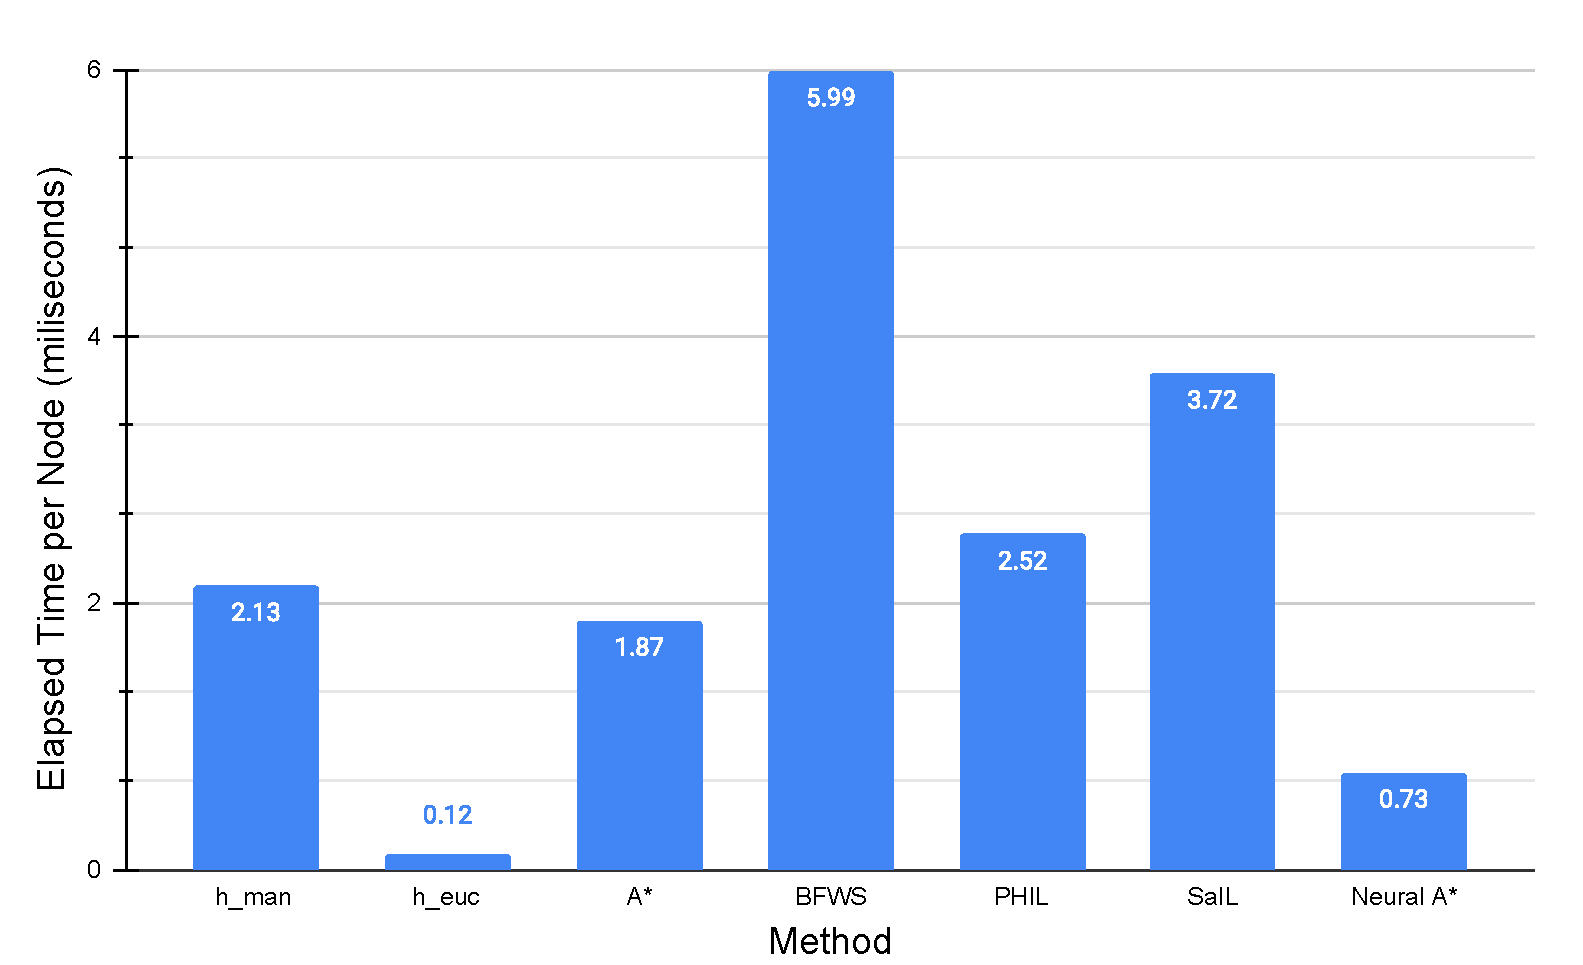
\includegraphics[width=0.9\linewidth]{PHIL/figures/runtime.pdf}
    \caption{Timing experiments on grid search datasets \cite{bhardwaj2017learning}.}
    \label{fig:phil-runtime}
\end{figure}

Figure~\ref{fig:phil-runtime} summarizes the test runtimes of the different approaches. PHIL runs $57.9\%$ faster than BFWS and $32.2\%$ faster than \sail , and not much slower than traditional A* ($34.7\%$) and $h_{man}$ ($18.3\%$). Although Neural A* is $71.0\%$ faster than PHIL due to the fact that it casts the whole search process into matrix operations on images, it cannot be employed in a generic search setting.
\section{Conclusion}

We consider the problem of learning to search for feasible paths in graphs efficiently. We propose a model and a training procedure to learn search heuristics that can be easily deployed across diverse graphs, with tuneable trade-off parameters between constant factors and performance. Our results demonstrate that \phil outperforms current state-of-the-art approaches and can be applied to various graphs with practical use cases.

\chapter{\dysta{}: Static-Dynamic Disentanglement for Efficient Multi-Frame Vision-Language-Action Models}
\label{chapter:dysta}

\section{Introduction}

Vision-Language-Action (VLA) models \cite{li2024cogact,kim2024openvla,qu2025spatialvla,kim2025fine,zhu2024surveymodelcompressionlarge,zhong2025surveyvisionlanguageactionmodelsaction,black2024pi0visionlanguageactionflowmodel,intelligence2025pi05visionlanguageactionmodelopenworld} have recently emerged as a powerful paradigm for generalist robotic control. Trained on large-scale heterogeneous datasets such as Open-X-Embodiment \cite{vuong2023open}, which aggregate expert demonstrations across diverse robotic tasks, state-of-the-art VLA models exhibit impressive task performance. However, they are typically built on top of large vision–language models \cite{liu2023visual,karamcheti2024prismatic,beyer2024paligemma,steiner2024paligemma}, whose large parameter counts and quadratic-complexity contextual processing \cite{vaswani2017attention} translate into two central deployment bottlenecks: (1) a constrained context budget that limits how many past observations can be ingested, and (2) high per-step inference latency that hinders real-time control. These manifest as the two challenges of \emph{multi-frame integration} and \emph{efficient inference} elaborated below and illustrated in Figure~\ref{fig:intro}.

\noindent\textbf{Multi-frame Integration}. Most current VLAs operate in a memoryless manner \cite{kim2024openvla,li2024cogact,qu2025spatialvla}, taking only the current observation as input. As a result, they struggle with tasks that require temporal dependency or memory tracking. For instance, when instructed to press a button, a VLA must remember whether the button has already been pressed; otherwise, it may repeat the same action indefinitely. A straightforward solution is to include previous observations in the model input. However, VLA's vision backbones typically produce hundreds of visual tokens per image, leading to prohibitively long contexts when multiple frames are concatenated for the transformer-based architecture with quadratic complexity in sequence length. Existing methods often rely on indirect or compressed representations \cite{jang2025contextvla,torne2026mem}, or expose multiple frames to the decoder head only \cite{shi2025memoryvlaperceptualcognitivememoryvisionlanguageaction}, which either risks significant information loss or bypasses the language model’s ability to jointly reason over multiple frames.

\noindent\textbf{Efficient Inference}. Due to their large model sizes, VLAs incur long latency for each forward pass. In real-world settings, however, robotic systems are often expected to respond promptly—for example, a household assistant should complete tasks as quickly as possible, while safety-critical scenarios such as spill containment or fire response may require near-instantaneous reactions. Moreover, recent post-training approaches for VLAs \cite{li2025simplevlarl,lu2025vla}, rely on reinforcement learning \cite{sutton1999policy,schulman2017proximal,shao2024deepseekmath} and require extensive rollouts during training, making inference speed a key bottleneck. While existing work has explored improving VLA efficiency through generic techniques for general machine learning models, such as quantization, token pruning, or layer pruning \cite{xu2025vla,yue2024deer,yang2025efficientvla,kim2024openvla}, these approaches do not leverage the intrinsic characteristics of VLA tasks. Recent works \cite{xu2025vla,liu2025ttf,tan2025think} exploit temporal redundancy by reusing computations across consecutive frames, via KV-cache reuse or action reuse. Nonetheless, these techniques rely on heuristic, non-learnable criteria and often assume that visual similarity in pixel space indicates the temporal-consistency of their latent representations—an assumption that is invalid in transformer-based vision and language backbones, as illustrated in Figure~\ref{fig:related_work1}.

\begin{figure}[t]
    \centering
    \includegraphics[width=\linewidth]{figs/teaser.pdf}
% \begin{subfigure}[b]{0.4\textwidth}
%     \centering
%     \includegraphics[height=7cm]{figs/teaser1.pdf}
%     \label{fig:0-input}
% \end{subfigure}
% \begin{subfigure}[b]{0.4\textwidth}
%     \centering
%     \includegraphics[height=7cm]{figs/teaser2.pdf}
%     \label{fig:0-input}
% \end{subfigure}
%     \caption{
%         Caption
%     }
\caption{Our model solves two main challenges in existing VLAs with the proposed static-dynamic disentanglement. 1) By keeping one copy of static tokens across all timesteps, our model is able to squash observations of multiple steps to the model's context; 2) By moving static tokens in front of all dynamic tokens, our model could reuse the KV-cache of previous timesteps during rollouts. }
    \label{fig:intro}
\end{figure}

To address these challenges, we propose \dysta{}. We focus on a broad and practically important class of robotic scenarios—such as tabletop manipulation, household chores, and warehouse picking—where the agent operates within relatively stable scenes or undergoes discrete, infrequent scene transitions. In this regime, much of the visual information in a scene remains static or changes slowly over time: the background, objects remaining still, and even moved objects whose visual appearances stay largely invariant. Building on this observation, we explicitly disentangle visual tokens into dynamic tokens and multi-level static tokens with different temporal persistence. This design yields two key benefits. First, instead of conditioning on a single image as in prior work, our model can ingest multi-step observations while maintaining a compact context: static tokens are included only once in the input sequence across timesteps, while only dynamic tokens from multiple steps are concatenated over time. This substantially reduces the effective context length and enables multi-frame integration. Second, our method improves the inference efficiency by reusing key–value (KV) caches associated with static tokens from previous steps. We also introduce a recache gate module that determines whether previously cached static tokens should be reused or recomputed, which further improves performance while minimizing the inference latency.

In addition, we observe that existing simulation benchmarks largely fail to assess a VLA's multi-frame integration capabilities. For example, temporally dependent tasks such as placing objects into a basket do not require remembering past trajectories. To address this gap, we design a new simulation benchmark inspired by principles of human episodic memory, which provides a more effective evaluation of temporal reasoning and memory usage than prior benchmarks \cite{liu2023libero,li2024evaluating}.

To evaluate multi-frame integration, we assess our model on the proposed benchmark. Our method achieves a $24.5\%$ improvement across all metrics and $23.3\%$ in absolute success rate on real-world experiments. To evaluate inference efficiency, we benchmark our approach on public simulation benchmarks~\cite{liu2023libero,li2024evaluating} and real-world experiments. On SimplerEnv~\cite{li2024evaluating}, \dysta{} improves the success rate by $3.9\%$ over the strongest baseline while achieving a $2.26\times$ inference speedup. In real-world experiments, \dysta{} improves the average success rate by $10.6\%$ over the base model and achieves a $2.21\times$ speedup. These results demonstrate that \dysta{} not only enhances multi-frame integration, but also substantially reduces inference latency. In summary, our contributions are as follows:

\begin{itemize}[noitemsep,topsep=0pt,leftmargin=*]
    \item We propose \dysta{}, which enables multi-frame integration and efficient inference by disentangling image tokens to dynamic tokens and multi-level static tokens with different temporal persistence.
    \item We introduce a trainable recache gate that adaptively determines when to refresh the cache or reuse previously cached representations, further improving the performance while minimizing the inference latency.
    \item We introduce LIBERO-Memory, a new benchmark that more effectively evaluates a VLA’s multi-frame integration ability by temporally dependent tasks.
\end{itemize}
\section{Related Works}

\noindent\textbf{Vision-Language-Action Models}
Vision-language models (VLMs) \citep{liu2023visual,wang2024cogvlm} have demonstrated strong performance in image-related and cross-modal tasks. Leveraging these capabilities, vision-language-action (VLA) models further finetune VLMs on large-scale robotic datasets \citep{vuong2023open,liu2023libero}, which usually consist of extensive human demonstrations. At each timestep, VLAs \citep{black2024pi0visionlanguageactionflowmodel,intelligence2025pi05visionlanguageactionmodelopenworld,kim2024openvla,li2024cogact,qu2025spatialvla} usually take the current environment observation (image) and a language instruction as inputs, and are trained to output actions of the next step. Although they have demonstrated high performance on certain benchmarks, due to the large parameters, they are 1) inefficient in rollout and 2) unable to incorporate historical frames in the context. In contrast, our model, by disentangling the static and dynamic components, is efficient in inference by leveraging the KV-cache of static components, and is able to incorporate a long history for temporally dependent tasks. 
\begin{figure}[t]
    \centering
    \includegraphics[width=0.8\linewidth]{figs/related_work1.pdf}
    \caption{Some of the existing methods \citep{xu2025vla,liu2025ttf} that exploit to reuse information in previous frames ignore the problem that the static patches will be affected by attentions even if they are identical in the original pixel space.}
    \label{fig:related_work1}
    % \vspace{-1em}
\end{figure}

\noindent\textbf{VLA Acceleration}
Methods to improve VLA's efficiency usually focus on general quantization or pruning methods. For example, \citet{kim2024openvla,reddy2019sqilimitationlearningreinforcement,park2024quantizationawareimitationlearningresourceefficientrobotic} explores quantization techniques applied to VLAs. \citet{shukor2025smolvlavisionlanguageactionmodelaffordable,yang2025efficientvla,zhang2025mole,yue2024deer} explored pruning unimportant tokens and layers according to some heuristics. Although reducing the computational complexity of VLAs, these methods just migrate acceleration methods from existing general machine learning models, thus totally ignoring the unique characteristics of VLAs. Different from these methods, recent works \citep{xu2025vla,liu2025ttf,tan2025think} explore temporal redundancy in decision making: consecutive frames share temporal correlation, enabling avoiding recomputation of some components by, for example, leveraging the KV-cache of previous steps. However, these methods rely on non-learnable heuristics to recache or simply reuse the previous action, which may suffer from suboptimal performance. Notably, some of these methods \citep{xu2025vla,liu2025ttf} implicitly assume that visual similarity in pixel space implies invariance in the latent representations produced by the vision encoder and LLM—an assumption that does not generally hold in transformer-based architectures, as illustrated in Figure~\ref{fig:related_work1}.

\noindent\textbf{Multi-Frame VLAs}
Existing approaches to incorporating historical frames in VLAs typically provide the model with only indirect or compressed access to temporal information. For example, \citet{jang2025contextvla} uses a non-learnable pooling operation to condense historical frames into a fixed number of tokens. \citet{liu2025ttf,torne2026mem} incorporate historical frames into the current input via patch-wise mixing. TraceVLA \citep{zheng2024tracevla} overlays visual traces of keypoints onto the current observation to indicate object trajectories. In addition, MemoryVLA \citep{shi2025memoryvlaperceptualcognitivememoryvisionlanguageaction} exposes the LLM backbone to only a single frame at each timestep and delegates multi-frame reasoning to a lightweight decoding module, which limits the model’s capacity for joint temporal decision-making. In contrast to these methods, our approach allows the LLM backbone to directly reason over multiple frames without information loss, by explicitly disentangling static and dynamic components and avoiding redundant involvement of temporally persistent visual information.
\section{Method}
In this section, we first present the problem formulation. We then introduce the architecture of our model, followed by the training objectives that enable static–dynamic disentanglement and the recaching mechanism. Next, we provide a computational complexity analysis and derive the theoretical acceleration and context-length improvements. Finally, we introduce the benchmark for evaluating multi-frame integration.

\noindent\textbf{Problem Formulation}
Given a timestep $t$, the corresponding observation of the environment is denoted by $\bs{X}_t$. A VLA $\pi$ predicts actions of the following steps based on previous $T$ observations and a language instruction $\mathcal{I}$.
\begin{equation}
    \pi: (\bs{X}_{t-T}, \bs{X}_{t-T+1}, \cdots, \bs{X}_{t}, \mathcal{I}) \mapsto \bs{a}_t, \bs{a}_{t+1}, \cdots,
\end{equation}

\begin{figure}[t]
    \centering
    \includegraphics[width=0.9\linewidth]{figs/arch.pdf}
    \caption{Model architecture overview. We illustrate the design using two levels of static cache. At each level, a recache gate determines whether the cached static tokens should be reused or refreshed. If the L1 cache is refreshed, the L2 cache is also forcibly refreshed.}
    \label{fig:dysta-arch}
    % \vspace{-1em}
\end{figure}


where $\bs{a}_t$ is the action at the $t$ step. Most existing VLAs usually consider $T=0$ due to the limited context length of large language models.


\subsection{Model Architecture}
\noindent\textbf{Static-dynamic disentanglement}
Standard VLA vision backbones typically encode the image $\bs{X}_t$ into $N$ image tokens $\bs{Z}_t=\bs{z}_{t,1}, \bs{z}_{t,2}, \cdots, \bs{z}_{t,N}$ as inputs of the VLA's LLM backbone $\pi_\text{LLM}$. Such a design implicitly assumes that all visual tokens must be recomputed and reprocessed at every timestep. However, real-world environments exhibit strong temporal redundancy: many visual attributes remain unchanged across time, while only a subset varies dynamically. Moreover, static information exists at different temporal scales. For example, global scene layout or background structure may persist for long horizons, whereas object-level appearance may change more frequently due to occlusion or interaction. To reflect this structure, we disentangle visual tokens into multi-level static tokens and dynamic tokens.

\begin{equation}
\bs{Z}^{s_1}_t, \bs{Z}^{s_2}_t, \cdots, \bs{Z}^d_t = \\
  \underbrace{\bs{z}_{t,1}, \cdots, \bs{z}_{t,N_{s_1}}}_\text{static tokens (level 1)}, \underbrace{\bs{z}_{t,1}, \cdots, \bs{z}_{t,N_{s_2}}}_\text{static tokens (level 2)}, \cdots, \underbrace{\bs{z}_{t,1}, \cdots, \bs{z}_{t, N_d}}_\text{dynamic tokens}
\end{equation}

where $\bs{Z}^{s_l}_t$ denotes static tokens at level $l$, and $\bs{Z}^{d}_t$ are dynamic tokens. The ratio between static and dynamic tokens is set as a predefined hyperparameter. Under this design, dynamic tokens capture timestep-specific information and are recomputed at every timestep, whereas static tokens at each level are selectively reused through a learned caching mechanism, described later.

\noindent\textbf{Temporal dependency modeling}
Most VLAs \cite{kim2024openvla,li2024cogact,qu2025spatialvla} are only able to process the current observation ($T=0$),
\begin{equation}
    \bs{a}_t, \bs{a}_{t+1}, \cdots = \pi_\text{LLM}(\bs{Z}_t),
\end{equation}
where $\pi_\text{LLM}$ is the LLM backbone of the VLA.
With successful static-dynamic disentanglement, we only need to keep \emph{one copy} of the static tokens within a period and construct the input from multiple observations as

\begin{equation}
    \bs{a}_t, \bs{a}_{t+1}, \cdots = \pi_\text{LLM}(\bs{Z}^{s_1}, \bs{Z}^{s_2}, \cdots,\bs{Z}^d_{t-T}, \cdots, \bs{Z}^d_t),
\end{equation}

This formulation enables the model to leverage longer temporal context without duplicating static information, effectively alleviating context window bottlenecks while preserving relevant visual cues.

\noindent\textbf{Learning when to recache}
A key challenge is deciding when cached static tokens should be refreshed. Naively recomputing static tokens at every timestep negates any computational benefit, while overly aggressive reuse of static tokens risks stale representations. To address this, we introduce a learned recache gate at each static level $l$,

\begin{equation}
    g_l(\bs{Z}_{t-\Delta}, \bs{Z}_t) \in [0, 1],\quad \Delta=1,2,\cdots, 
\end{equation}

which predicts the probability that static tokens should be recomputed given the current observation and a cached reference from $\Delta$ timesteps earlier. During training, we use the Gumbel-softmax trick \cite{jang2016categorical,maddison2016concrete} to allow end-to-end differentiable binary decisions. At inference time, static tokens are refreshed if the probability is greater than a threshold, i.e., $g_l > \delta_l$; otherwise, the previous cache is reused. It is also worth noting that if the higher-level cache (e.g., L1) should be refreshed, the lower-level cache (e.g., L2) should also be refreshed during both training and inference. Additional details of the architecture of the recache gate could be found in Appendix~\ref{app:arch}.


\noindent\textbf{Computational and Acceleration Analysis}
Let $N$ be the total number of tokens per observation, $r$ the fraction of cached static tokens, and $T$ the number of observations in the context. Our static-dynamic disentanglement reduces the effective context length from $NT$ to $NT - rN(T-1)$, and reduces the FLOPs of the LLM backbone by a factor of $1-r$. The recache gate adds only negligible overhead ($\approx 1.27\%$). A full derivation and wall-clock latency breakdown are provided in Appendix~\ref{app:complexity}.

\begin{figure}[t]
    \centering
    \includegraphics[width=0.5\linewidth]{figs/contrastive.pdf}
    \caption{Contrastive loss used to train static tokens to be temporally persistent. Observations from the same trajectory form positive pairs, while observations from different trajectories form negative pairs.}
    \label{fig:contrastive}
    % \vspace{-1em}
\end{figure}

\subsection{Training Objective}


Besides the standard task loss of the underlying VLA base model $\mathcal{L}_\text{task}$, we introduce two additional training objectives. The first promotes temporally persistent static tokens, and the second trains the cache gate that adaptively determines when cached representations should be refreshed.

\noindent\textbf{Learning static tokens} As illustrated in Figure~\ref{fig:contrastive}, to ensure that static tokens can be safely and effectively reused across time, they must remain stable over a temporal window while still encoding task-relevant information. To encourage this property, we apply a contrastive term to the static tokens. Specifically, observations from different timesteps within the same trajectory are treated as positive pairs, while observations from different trajectories are treated as negative pairs. We employ InfoNCE loss~\cite{oord2018representation} $\mathcal{L}_{\text{InfoNCE}}^{l}$ to perform contrastive learning for static tokens at level $l$.



% \begin{equation}
% \begin{aligned}
%     &\mathcal{L}_\text{InfoNCE}^l= \\
%     &\frac{1}{TN_{s_l}} \sum_{\Delta=1}^T \sum_{i=1}^{N_{s_l}} \frac{\exp(\bs{z}^{s_l}_{t,i} \cdot \bs{z}^{s_l}_{t-\Delta, i})}{\exp(\bs{z}^{s_l}_{t,i} \cdot \bs{z}^{s_l}_{t-\Delta, i}) + \sum_{z^-}\exp(\bs{z}^{s_l}_{t,i} \cdot \bs{z}_{}^-)},
% \end{aligned}
% \end{equation}
% where $N_{s_l}$ is the number of static tokens at level $l$. $\bs{z}^-$ are negative samples (i.e., observations from different trajectories). 

% Optimizing this objective encourages static tokens to remain consistent across timesteps within a trajectory, thereby making cache reuse safer and more effective during inference.

\noindent\textbf{Training the recache gate}
If the recache gate is trained only through task supervision, it tends to recompute static tokens at every timestep, which eliminates any computational benefit. To discourage this trivial solution, we add a regularization term that biases the gate toward reuse when observations are close in time.

\begin{equation}
    \mathcal{L}_\text{gate} = -p_\Delta \log g - (1-p_\Delta)\log (1-g),
\end{equation}

where $p_{\Delta} = 1 - e^{-\lambda \Delta}$ is a predefined prior which allows the use of current observation only when $\Delta$ is large. The recache gate learns to adaptively refresh static tokens only when necessary, balancing computational efficiency and model performance. Note that since $\lambda$ and the recache threshold $\delta_l$ jointly determine the recaching frequency, we fix $\lambda$ and expose only $\delta_l$ as the operating-point knob. 

The full training objective is
\begin{equation}
    \mathcal{L} = \mathcal{L}_\text{Task} + \sum_l \alpha_l  \mathcal{L}^l_\text{InfoNCE} + \beta \mathcal{L}_\text{gate},
\end{equation}
where $\alpha_l$ and $\beta$ weight the auxiliary regularization terms. A sensitivity analysis for these coefficients is provided in Appendix~\ref{app:sense}.

\subsection{LIBERO-Memory Benchmark}

Existing VLA simulation benchmarks \cite{liu2023libero, li2024evaluating} are designed for memoryless tasks, which do not require multi-frame integration, and the current observation alone is theoretically sufficient to predict the next action. For example, in a task with the goal “put X in the basket”, \cite{liu2023libero} the agent can act optimally without retaining information from previous frames. As a result, it is unclear whether the reported performance of existing models for modeling temporal dependency \cite{jang2025contextvla,shi2025memoryvlaperceptualcognitivememoryvisionlanguageaction} truly stems from improved temporal modeling or from other artifacts. This highlights the absence of a strong and fair benchmark for temporal dependency modeling and multi-frame integration.

To address this gap, we introduce a new simulation benchmark designed to test multi-frame integration explicitly. Our benchmark includes tasks that require a robot to retain and utilize information from past observations, thereby directly evaluating a model's temporal dependency modeling ability.

Following the setup of LIBERO, the robot operates in a tabletop environment containing three objects: two visually distinct cans and a stove. As illustrated in Figure~\ref{fig:libero_stove}, each episode consists of three tasks which reflects the structure of episodic memory \cite{tulving1972episodic,clayton1998episodic}.

\begin{figure}[t]
    \centering
    \includegraphics[width=\linewidth]{figs/libero_stove.pdf}
    \caption{An example of the procedure of the proposed benchmark. }
    \label{fig:libero_stove}
    % \vspace{-1em}
\end{figure}


\noindent\textbf{Tasks}
Each trial consists of three subtasks, each intentionally designed to require the model to retain and reason over information from previous observations at different aspects: 1) Grasp one of the cans, as specified by the instruction, and place it on the stove to heat. 2) After a period of time (given in the instructions), remove the can from the stove and return it to its original location. 3) Once the position of the first can has been restored, grasp the remaining can and place it on the stove.

This task design requires the model to retain \emph{episodic memory}, integrating information about what happened, where it occurred, and when it took place \cite{tulving1972episodic,clayton1998episodic}. First, the robot must remember the initial spatial layout in order to return the first can to its original position (where). Second, it must track the elapsed time since the can was placed on the stove to determine when to remove it (when). Third, it must remember which can has already been heated in order to correctly select the remaining one for the final step (what).

These requirements prevent the task from being solved using only the current observation or a short observation history. We use Robosuite \cite{zhu2025robosuitemodularsimulationframework} as the simulation framework to produce the dataset. The layout and the oracle demonstrations are programmatically generated. More details can be found in Appendix \ref{app:dataset_memory}.

\section{Experiments}
In this section, we evaluate the model’s inference efficiency as well as its multi-frame integration ability. We further present ablation studies of the key components of our method and analyze the model’s behavior through attention-map visualizations.


\subsection{Acceleration}
In this study, we validate our method's performance under acceleration by enabling KV caching of static components. 

\noindent\textbf{Baselines}
For baselines, we compare to those that also adopt temporal information reuse. \emph{FlashVLA} \cite{tan2025think} simply reuses the previous action based on a heuristic criterion.
\emph{TTF-VLA} \cite{liu2025ttf} and \emph{VLA-cache} \cite{xu2025vla} identify reusable visual patches using hand-designed heuristics and cache the corresponding embeddings from previous steps; however, these cached patches are not guaranteed to remain static in the hidden representation space. All methods are based on the same VLA base model (i.e., CogACT~\cite{li2024cogact}), with all other necessary variables controlled consistently.

% \begin{table*}[]
% \newcolumntype{M}{>{\raggedleft\arraybackslash}p{0.1\linewidth}}
% \newcommand{\cchead}[1]{\multicolumn{1}{c}{#1}}
%     \centering\textbf{}
% \caption{Results on the SimplerEnv benchmark.}
% \label{tab:simplerenv}
%     \resizebox{\linewidth}{!}{
% \begin{tabular}{l|l|ccccc|ccc}
% \toprule
%  Google Robot & Method & PickCan & MoveNear & Drawer & DrawerApple & Average & FLOPs & Latency (ms) & Speedup \\
%  \midrule
%  \multirow{5}{*}{\makecell{SIMPLER\\ (Visual Matching)}}
%  & CogACT \cite{li2024cogact} & $91.3$ & $85.0$ & $71.8$ & $50.9$ & $74.8$ & 100\% & $339$ & $1.00\times$ \\
%   & + FlashVLA \cite{tan2025think} & $80.0$ & $57.1$ & $73.6$ \\
%  % RT-1 & 85.7 & 44.2 & 73.0 & 6.5 & 52.4 & NA \\
%  % & RT-1-X & 56.7 & 31.7 & 59.7 & 21.3 & 42.4 \\
%  % & RT-2-X  & 78.7 & 77.9 & 25.0 & 3.7 & 46.3 & NA \\
%  % & Octo-Base  & 17.0 & 4.2 & 22.7 & 0.0 & 11.0 & NA \\
%  % & OpenVLA  & 18.0 & 56.3 & 63.0 & 0.0 & 34.3 & NA \\
%  & + TTF \cite{liu2025ttf} & $89.3$ & $71.3$ & $58.4$  \\
%  & + VLA-Cache \cite{xu2025vla} &  $92.0$ & $85.0$  & $70.5$ & $51.6$ & & $80.1\%$ \\
%  % & EfficientVLA & 93.3 & 81.3 & 68.2 & 53.8 & 28.9\% \\
%  & + \dysta{} (Ours) & $92.7$ & $88.8$ & $75.0$ & $47.2$ & & $40.2\%$ & $151$ \\
%  \midrule
%  \multirow{5}{*}{\makecell{SIMPLER\\ (Variant Aggregation)}}
%  & CogACT \cite{li2024cogact} & $89.6$ & $80.8$ & $28.3$ & $46.6$ & $61.3$ \\
%  & + FlashVLA \cite{tan2025think} & $82.5$ & $60.8$ & $28.6v$\\
%  % & RT-1 [7] & 89.8 & 50.0 & 32.3 & 2.6 & 43.7 \\
%  % & RT-1-X [48] & 49.0 & 32.3 & 29.4 & 10.1 & 30.2 \\
%  % & RT-2-X [48] & 82.3 & 79.2 & 35.3 & 20.6 & 54.4 \\
%  % & Octo-Base [62] & 0.6 & 3.1 & 1.1 & 0.0 & 1.2 \\
%  % & OpenVLA [30] & 60.8 & 67.7 & 28.8 & 0.0 & 39.3 \\
%  & + TTF \cite{liu2025ttf} & $88.0$ & $62.7$ & $34.0$ \\
%  & + VLA-Cache \cite{xu2025vla} & $91.7$ & $79.3$  & $32.5$ & $45.8$ & \\
%  % & EfficientVLA & 93.2 & 75.8 & 26.9 & 49.2 & \\
%  & + \dysta{} (Ours) & $92.4$ & $81.0$ & $38.9$ & $46.0$ & \\
%  \bottomrule
% \end{tabular}
% }
% \end{table*}


% \begin{table*}[t]
% \newcolumntype{M}{>{\raggedleft\arraybackslash}p{0.1\linewidth}}
% \newcommand{\cchead}[1]{\multicolumn{1}{c}{#1}}
%     \centering\textbf{}
% \caption{Results on the SimplerEnv benchmark. Task suites follows the setting of \citet{qu2025spatialvla}.}
% \label{tab:simplerenv}
%     \resizebox{\linewidth}{!}{
% \begin{tabular}{l|cccccccc|ccc}
% \toprule
% \multirow{3}{*}{Method} & \multicolumn{4}{c}{Visual Matching} & \multicolumn{4}{c}{Variant Aggregation} & \multicolumn{3}{c}{Acceleration}  \\
% \cmidrule(lr){2-5}\cmidrule(lr){6-9}\cmidrule(lr){10-12}
% & \makecell{Pick\\Can} & \makecell{Move\\Near} & Drawer & \makecell{Drawer\\Apple} & \makecell{Pick\\Can}  & \makecell{Move\\Near} & Drawer & \makecell{Drawer\\Apple}   & FLOPs & \makecell{Latency\\(ms)} & Speedup \\
%  \midrule
%  CogACT \cite{li2024cogact} & $91.3$ & $85.0$ & $71.8$ & $50.9$ &$89.6$ & $80.8$ & $28.3$ & $46.6$  & 100\% & $1355$ & $1.00\times$ \\
%   + FlashVLA \cite{tan2025think} & $80.0$ & $57.1$ & $73.6$ & & $82.5$ & $60.8$ & $28.6$ &\\
%  + TTF \cite{liu2025ttf} & $89.3$ & $71.3$ & $58.4$ & & $88.0$ & $62.7$ & $34.0$ & \\
%  + VLA-Cache \cite{xu2025vla} &  $92.0$ & $83.3$  & $70.5$ &  & $91.7$ & $79.3$  & $32.5$ & $45.8$ & $80.1\%$ \\
%  + \dysta{} (Ours) & $\mathbf{92.7}$ & $\mathbf{88.8}$ & $\mathbf{75.0}$ & $47.2$ & $\mathbf{92.4}$  & $\mathbf{81.0}$ & $\mathbf{38.9}$ & $46.0$& $43.4\%$ & $577$ & $2.35\times$ \\
%  \bottomrule
% \end{tabular}
% }
% \end{table*}


\begin{table}[t]
\newcolumntype{M}{>{\raggedleft\arraybackslash}p{0.1\linewidth}}
\newcommand{\cchead}[1]{\multicolumn{1}{c}{#1}}
    \centering\textbf{}
\caption{Results on the SimplerEnv benchmark. Task suites follow the setting of \citet{qu2025spatialvla}. All baselines and our method are applied to the same VLA base model (i.e., CogACT~\cite{li2024cogact}).}
\label{tab:simplerenv}
    \resizebox{\linewidth}{!}{
\begin{tabular}{lcccccc|ccc}
\toprule
\multirow{3}{*}{Method} & \multicolumn{3}{c}{Visual Matching} & \multicolumn{3}{c}{Variant Aggregation} & \multicolumn{3}{c}{Acceleration}  \\
\cmidrule(lr){2-4}\cmidrule(lr){5-7}\cmidrule(lr){8-10}
& \makecell{Pick\\Can} & \makecell{Move\\Near} & Drawer & \makecell{Pick\\Can}  & \makecell{Move\\Near} & Drawer  & FLOPs & \makecell{Latency\\(ms)} & Speedup \\
 \midrule
  % RT-2-X \cite{vuong2023open} & $78.7$ & $77.9$ & $25.0$ & $82.3$ & $79.2$ & $35.3$ & $-$ & $-$ & $-$\\
  % Octo-Base \cite{team2024octo} & $17.0$ & $4.2$ & $22.7$ & $0.6$ & $3.1$ & $1.1$ & $-$ & $-$ & $-$ \\
  % OpenVLA \cite{kim2024openvla}  & $18.0$ & $56.3$ & $63.0$ & $60.8$ & $67.7$ & $28.8$ & $-$ & $-$ & $-$ \\
  % SpatialVLA \cite{qu2025spatialvla} & $81.0$ & $69.6$ & $59.3$ & $89.5$ & $71.7$ & $36.2$ & $-$ & $-$ & $-$ \\
  % $\pi_0$ \cite{black2024pi0visionlanguageactionflowmodel} & $88.0$ & $80.3$ & $56.0$ & $-$ & $-$ & $-$ & $-$ & $-$ & $-$ \\
  % \midrule
 CogACT \cite{li2024cogact} & $91.3$ & $\underline{85.0}$ & $71.8$ &$89.6$ & $\underline{80.8}$ & $28.3$  & 100\% & $1360$ & $1.00\times$ \\
  + FlashVLA \cite{tan2025think} & $80.0$ & $57.1$ & $\underline{73.6}$ & $82.5$ & $60.8$ & $28.6$ & $83.4\%$ & $1024$ & $1.33\times$\\
 + TTF \cite{liu2025ttf} & $89.3$ & $71.3$ & $58.4$ & $88.0$ & $62.7$ & $\underline{34.0}$ & $86.5\%$ & $1051$ & $1.29\times$  \\
 + VLA-Cache \cite{xu2025vla} &  $\underline{92.0}$ & $83.3$  & $70.5$ & $\underline{91.7}$ & $79.3$  & $32.5$ & $80.1\%$ & $985$ & $1.38\times$ \\
 + \dysta{} (Ours) & $\mathbf{92.7}$ & $\mathbf{88.8}$ & $\mathbf{75.0}$ & $\mathbf{92.4}$  & $\mathbf{81.0}$ & $\mathbf{38.9}$ & $\mathbf{43.4\%}$ & $\mathbf{601}$ & $\mathbf{2.26\times}$ \\
 \bottomrule
\end{tabular}
}
\end{table}


\begin{table}[t]
\centering
\caption{Results on the LIBERO benchmark. Policy inputs: third-person image, language instruction. All baselines and our method are applied to the same VLA base model (i.e., OpenVLA-OFT~\cite{kim2025fine}).}
\label{tab:libero}
\resizebox{\linewidth}{!}{
\begin{tabular}{lccccc|ccc}
\toprule
Models & Spatial & Object & Goal & Long & Average & FLOPs & Latency (ms) & Speedup \\
\midrule
% Diffusion Policy \cite{chi2025diffusion} & 78.3 & 92.5 & 68.3 & 50.5 & 72.4 & $-$ & $-$& $-$ \\
% Octo \cite{team2024octo} & 78.9 & 85.7 & 84.6 & 51.1 & 75.1 & $-$ & $-$& $-$\\
% DiT Policy \cite{hou2410diffusion} & 84.2 & 96.3 & 85.4 & 63.8 & 82.4 & $-$ & $-$& $-$\\
% OpenVLA \cite{kim2024openvla} & 84.7 & 88.4 & 79.2 & 53.7 & 76.5 & $-$ & $-$& $-$\\
% \midrule
OpenVLA-OFT \cite{kim2025fine} & $\underline{96.2}$ & $\mathbf{98.3}$ & $\mathbf{96.2}$ & $\underline{90.7}$ & $\underline{95.4}$ & $100.0\%$ & $741$ & $1.00\times$\\
% \midrule
+ FlashVLA \cite{tan2025think} & $71.8$ & $90.0$ &  $79.2$& $78.8$ & $80.0$ &  $88.7\%$& $657$ & $1.13\times$  \\
+ TTF \cite{liu2025ttf} & $95.8$ & $94.2$ &   $93.6$ &  $86.0$  & $92.4$ & $75.0\%$ & $575$ & $1.29\times$\\
% EfficientVLA & & & & 89.8 & \\
+ VLA-Cache \cite{xu2025vla} & $95.6$ & $92.8$ & $94.0$ & $89.6$ & $93.0$ & $85.5\%$ & $652$ & $1.14\times$ \\
+ \dysta{} (Ours) & $\mathbf{97.8}$ & $\underline{97.6}$ & $\mathbf{96.2}$ & $\mathbf{92.4}$ & $\mathbf{96.0}$ & $\mathbf{63.4}\%$ & $\mathbf{437}$ & $\mathbf{1.70}\times$ \\
\bottomrule
\end{tabular}
}
\end{table}

\noindent\textbf{Simulation benchmark}
We use SimplerEnv~\cite{li2024evaluating} and LIBERO~\cite{liu2023libero} task suite to evaluate the performance and acceleration. \citet{kim2025fine} offers two settings for LIBERO, one using only a third-person image and a language instruction as inputs, and another that additionally includes an extra camera view and proprioceptive state. We adopt the former setting, as it offers broader applicability and aligns more closely with standard VLA deployment scenarios. For the LIBERO benchmark, we finetune the model to the corresponding downstream datasets. For the SimplerEnv benchmark, we use Open X-Embodiment (OXE) \cite{vuong2023open} as the training dataset. All settings are consistent with the corresponding original base model.

\noindent\textbf{Real-World benchmark} We evaluate \dysta{} with Cobot Magic robots on 7 tasks across 3 categories, each with 20 trials. This evaluation scale is consistent with prior work~\cite{shi2025memoryvlaperceptualcognitivememoryvisionlanguageaction,li2024cogact}.

\noindent\textbf{Evaluation} The performance is measured by success rate, and acceleration is measured by the FLOPs reduction rate and the inference latency.

\noindent\textbf{Implementation details} We use two levels of static cache. L1 static cache consists of 133 ($52\%$) tokens and L2 static cache consists of 107 ($42\%$) tokens, resulting in 16 dynamic tokens. FLOPs are measured by open-source tools \footnote{\url{https://github.com/MrYxJ/calculate-flops.pytorch}}.

\noindent\textbf{Results}
Table~\ref{tab:simplerenv}  and Table~\ref{tab:libero} summarize the performance and the acceleration results. Table~\ref{tab:real_res} summarizes the results on the real-world benchmark. Across tables, we show that our method achieves improved or comparable performance across benchmarks with substantial speedup. Notably, on the SimplerEnv benchmark, our method improves the base model by $4.9\%$, and outperforms the best baseline by $3.9\%$ and achieves $2.26\times$ acceleration.  On the real-world benchmark, our model improves the base model by $10.6\%$ and achieves $2.21\times$ acceleration.

\subsection{Multi-Frame Integration for Temporal-dependency Modeling} 

\noindent\textbf{Baselines}
We consider the following baselines: \emph{OpenVLA-OFT$^\dagger$} incorporates full image tokens from historical observations. Since this baseline incurs a prohibitively large context length compared with standard models, we allocate the maximum available resources and tune it for the best achievable performance. \emph{TTF-VLA} \cite{liu2025ttf} mixes the current observation with past observations in a patch-wise manner. \emph{TraceVLA} \cite{zheng2024tracevla} visualizes the trajectories of active points by overlaying them onto the image using distinct colors, referred to as visual traces. \emph{MemoryVLA} \cite{shi2025memoryvlaperceptualcognitivememoryvisionlanguageaction} feeds the LLM backbone with images from each timestep independently and extracts a representation for each; only the multi-timestep representations are provided to the decoder. \emph{ContextVLA} \cite{jang2025contextvla} pools historical observations into a fixed number of tokens and prepends them to the image tokens of the current observation. All methods are applied to the same VLA base model (i.e., OpenVLA-OFT~\cite{kim2025fine}), with all other necessary variables controlled consistently.


\begin{table}[t]
\centering
\caption{Success rate (\%) on real-world experiments with the Cobot Magic robot. All baselines and our method are applied to the same VLA base model (i.e., OpenVLA-OFT~\cite{kim2025fine}).}
\label{tab:real_res}
\resizebox{\linewidth}{!}{
\begin{tabular}{l|cccc|cc|c|ccc}
\toprule
\multirow{3}{*}{Method}
& \multicolumn{4}{c|}{Pick-and-Place}
& \multicolumn{2}{c|}{Pouring}
& \multicolumn{1}{c|}{Container}
& \multicolumn{3}{c}{Acceleration Metrics} \\
\cmidrule(lr){2-5}
\cmidrule(lr){6-7}
\cmidrule(lr){8-8}
\cmidrule(lr){9-11}

& \makecell{Corn\\$\rightarrow$Pot}
& \makecell{Corn\\$\rightarrow$Plate}
& \makecell{Bread\\$\rightarrow$Pan}
& \makecell{Carrot\\Transfer}
& \makecell{Pour\\Coke}
& \makecell{Pour\\Bottle}
& \makecell{Open\\Drawer}
& FLOPs
& \makecell{Latency\\(ms)}
& Speedup \\
\midrule

OpenVLA-OFT
& $55$ & $\underline{70}$ & $\mathbf{55}$ & $\underline{65}$
& $\underline{60}$ & $35$
& $\mathbf{35}$
& $100.0\%$
& $1089$
& $1.00\times$ \\

+ FlashVLA
& $35$ & $55$ & $30$ & $50$
& $55$ & $30$
& $15$
& $\underline{62.5\%}$
& $\underline{791}$
& $\underline{1.30\times}$ \\

+ TTF
& $35$ & $\underline{70}$ & $30$ & $55$
& $55$ & $\underline{40}$
& $15$
& $98.6\%$
& $1077$
& $1.01\times$ \\

+ VLA-Cache
& $\underline{60}$ & $65$ & $35$ & $50$
& $45$ & $\underline{40}$
& $30$
& $74.0\%$
& $836$
& $1.27\times$ \\

% \midrule
+ \dysta{} (Ours)
& $\mathbf{65}$ & $\mathbf{80}$ & $\underline{50}$ & $\mathbf{70}$
& $\mathbf{60}$ & $\mathbf{50}$
& $\mathbf{35}$
& $\mathbf{30.5\%}$
& $\mathbf{493}$
& $\mathbf{2.21\times}$ \\
\bottomrule
\end{tabular}
}
\end{table}

\noindent\textbf{Simulation benchmark and evaluation} We adopt the proposed LIBERO-memory benchmark to evaluate multi-frame integration by memory-dependent tasks, whose designs are inspired by the notion of episodic memory. The benchmark comprises three objectives.
(1) \emph{(where) Position Reset.} After heating the first can, the robot is required to remember its original position and return it to the position. Performance is measured by success rate, where an episode is considered successful if the positional error is below a threshold.
(2) \emph{(when) Doneness.} The model must track the elapsed heating time and remove the can at the appropriate moment. Given a target heating duration specified in the instruction, we measure the absolute difference (in seconds) between the actual and desired heating times, capturing overcooking or undercooking.
(3)\emph{(what) On-Stove.} After heating and resetting the first can, the robot is required to remember which can has been cooked and place the second can on the stove for heating. We report the success rate of placing the second can on the stove.

\begin{table}[t]
    \centering
    \caption{Results on the temporal-dependent tasks for multi-frame integration. All models use OpenVLA-OFT \cite{kim2025fine} as the base model. OpenVLA-OFT$^\dagger$ denotes a naive baseline that packs as many frames as possible into the context.}
    \label{tab:stove_res}
    \resizebox{\linewidth}{!}{
    \begin{tabular}{lccc}
    \toprule
        Models & On Stove $\uparrow$ & Position Reset $\uparrow$ & Doneness (seconds) $\downarrow$ \\
    \midrule
        OpenVLA-OFT$^\dagger$ & $39.0\%$ & $78.0\%$ & $0.44$ \\
        TTF-VLA \cite{liu2025ttf} & $7.8\%$ & $1.5\%$ & $1.51$ \\
        TraceVLA \cite{zheng2024tracevla} & $2.0\%$ & $3.0\%$ & $1.41$ \\
        MemoryVLA \cite{shi2025memoryvlaperceptualcognitivememoryvisionlanguageaction} & $23.0\%$ & $2.0\%$ & $1.49$ \\
        ContextVLA \cite{jang2025contextvla} & $50.8\%$ & $22.3\%$ & $0.37$ \\
        \dysta{} (Ours) & $\mathbf{69.8}\%$ & $\mathbf{83.0}\%$ &  $\mathbf{0.26}$ \\
    \bottomrule
    \end{tabular}
    }
\end{table}



\noindent\textbf{Real-world benchmark}
We evaluated \dysta{} with Cobot Magic robots on three tasks requiring memory or temporal reasoning. In \emph{Heat Vegetables}, the robot heated vegetables one at a time and had to remember which had already been heated. In \emph{Pour Twice}, it had to track whether the first pour had been completed. In \emph{Press Buttons}, it had to remember which buttons had already been pressed and determine the next button in the sequence. We varied the objects' locations and the robot arm's starting position. Models were finetuned on each task, and performance was measured by success rate over 20 trials per task. Figure~\ref{fig:dysta-real-mem} illustrates the three tasks.

\begin{figure}[htbp]
    \centering
    \includegraphics[width=\linewidth]{figs/real_demo_mem.jpg}
    \caption{Real-world tasks for multi-frame integration with the Cobot Magic robot: Press Buttons (top), Pour Twice (middle), and Heat Vegetables (bottom). Each task was evaluated over 20 trials.}
    \label{fig:dysta-real-mem}
\end{figure}

\begin{table}[t]
\centering
\caption{Real-world task accuracy (\%) on temporally dependent tasks for multi-frame integration. Each task is evaluated over 20 trials.}
\label{tab:real_mem}
\begin{tabular}{l|ccc|c}
\toprule
Method
& \makecell{Heat\\Vegetables}
& \makecell{Pour\\Twice}
& \makecell{Press\\Buttons}
& Average \\
\midrule
MemoryVLA
& $10.0$
& $25.0$
& $45.0$
& $26.7$ \\
ContextVLA
& $25.0$
& $40.0$
& $40.0$
& $35.0$ \\
\dysta{} (Ours)
& $\mathbf{35.0}$
& $\mathbf{75.0}$
& $\mathbf{65.0}$
& $\mathbf{58.3}$ \\
\bottomrule
\end{tabular}
\end{table}


\noindent\textbf{Implementation details} We use one static level. The ratio of static tokens is set to $0.9$, corresponding to $230$ static tokens and $26$ dynamic tokens. The number of observations is set to $20$, with a sampling interval of $20$ frames (1 frame per second), resulting in $750$ context tokens.


\noindent\textbf{Results} 
As shown in Table~\ref{tab:stove_res}, our method significantly and consistently outperforms all baselines on all objectives, with an average improvement of $24.5\%$.
Single-image methods such as TraceVLA almost always fail, since the task cannot be solved from the current observation alone, and visual traces provide only marginal additional benefit. 
ContextVLA underperforms due to non-learnable pooling observations, which may discard critical temporal and spatial details.
MemoryVLA presents the LLM backbone with only a single frame at each timestep, leaving multi-frame reasoning to a lightweight decoder; as a result, the LLM itself does not reason over multiple frames, which limits the model's capacity.
While these baselines have their own ways to reduce context length, they do so at the cost of information or model capacity. In contrast, our approach preserves all relevant visual information by reusing temporally persistent static tokens, enabling effective multi-frame integration within a limited context window.

\noindent\textbf{Real-world results}
As shown in Table~\ref{tab:real_mem}, \dysta{} achieved an average success rate of $58.3\%$ across the three real-world tasks, outperforming ContextVLA, the strongest baseline on average ($35.0\%$), by $23.3$ percentage points.

\subsection{Ablation Studies}

To validate the effectiveness of the proposed components, we conduct ablation studies on each of them, with results summarized in Table~\ref{tab:dysta-ablation}. From the second row, removing the contrastive learning objective leads to a noticeable performance degradation, as there is no longer an explicit mechanism to enforce temporal consistency in the static tokens. Performance also declines when the L2 static cache is removed and only a single-level static cache is used, as shown in the third row, highlighting the importance of the proposed multi-level caching design. Finally, replacing the learnable recache gate results in a further drop in performance, demonstrating the necessity of adaptive cache refreshing.

\begin{table}[t]
    \centering
        \caption{Ablation studies. \emph{w/o Contrast} removes the contrastive learning objective during training. \emph{w/o L2 cache} ablates the multi-level design by retaining only a single static cache level. \emph{Fixed step} replaces the learnable recache gate by forcing the refresh of the cache at fixed intervals. The refresh interval is set to match the average recaching interval of \dysta{} (first row).}
    \label{tab:dysta-ablation}
    \resizebox{\linewidth}{!}{
    \begin{tabular}{cccccc}
    \toprule
         & \multicolumn{2}{c}{visual matching} && \multicolumn{2}{c}{variant aggregation}  \\
         \cmidrule{2-3}
         \cmidrule{5-6}
         & PickCan & MoveNear & & PickCan & MoveNear \\
         \midrule
        \dysta{} & $\mathbf{92.7}$ & $\mathbf{88.8}$ & &$\mathbf{92.4}$ & ${81.0}$ \\ 
        w/o Contrast & $91.3$ & $84.6$ & &$91.6$ & $\mathbf{82.7}$ \\
        w/o L2 cache & $92.0$ & $85.0$ & & $91.5$ & $81.5$ \\
        fixed step & $87.7$ & $81.7$ & & $85.3$ & $74.8$ \\
    \bottomrule
    \end{tabular}
    }
\end{table}

\subsection{Visualizations}
We visualize the attention between the image and static/dynamic tokens across timesteps in Figure~\ref{fig:attention}.

\begin{figure}[t]
    \centering
    \includegraphics[width=0.9\linewidth]{figs/vis.pdf}
% \vspace{-15pt}
    \caption{Attention map visualization across time. For each token, we compute its last-layer attention to image patches and upsample the result to the full image resolution to produce a heatmap. Heatmaps are averaged over tokens of the same type and displayed by row (e.g., the Dynamic row shows the average attention heatmap of all dynamic tokens).}
    \label{fig:attention}
\end{figure}
Dynamic tokens consistently attend to movable objects, most notably the gripper (including its shadow) and the apple on the tabletop. This behavior aligns with their intended role of capturing temporally varying, action-relevant elements in the scene.

L1 static tokens, which are designed to represent the most persistent visual information, primarily focus on background and ambient regions. Their attention heatmaps are often strongest in areas without salient foreground objects. We interpret this behavior as L1 static tokens of shallow layers functioning as sink tokens, capturing coarse, global scene context rather than object-specific details. Importantly, their attention patterns remain highly consistent across timesteps, reflecting strong temporal invariance.

L2 static tokens exhibit intermediate behavior between L1 static and dynamic tokens. They attend more strongly to semi-static objects, such as the drawer, which typically remains stationary most of the time. At $t=0$ both drawer handles are highlighted, as either could potentially be moved. After the drawer is opened ($t>100$), the attention maps stabilize and remain focused on the drawer structure, indicating that these tokens capture object-level static information with moderate temporal persistence. The robotic arm is also highlighted at certain frames, which we attribute to its importance in the task and the need to preserve its appearance across timesteps.


\section{Conclusion}
We introduced \dysta{}, a method that improves efficiency and multi-frame integration in VLA models via static–dynamic disentanglement. By reusing temporally persistent static tokens and selectively refreshing them through a learnable recache gate, \dysta{} enables compact multi-frame contexts and efficient inference. Experiments show that our approach substantially improves performance on temporally dependent tasks while providing meaningful speedups over strong baselines. These results suggest that explicitly modeling temporal persistence is a promising direction for scalable and practical VLA systems. \noindent\textbf{Limitations}. We realize our approach based on pretrained VLAs. Such a strategy may not fully unleash the performance of the model. Future work could focus on pretraining VLAs with our architecture from scratch.

